\documentclass{tufte-handout}\usepackage[]{graphicx}\usepackage[]{xcolor}
% maxwidth is the original width if it is less than linewidth
% otherwise use linewidth (to make sure the graphics do not exceed the margin)
\makeatletter
\def\maxwidth{ %
  \ifdim\Gin@nat@width>\linewidth
    \linewidth
  \else
    \Gin@nat@width
  \fi
}
\makeatother

\definecolor{fgcolor}{rgb}{0.345, 0.345, 0.345}
\newcommand{\hlnum}[1]{\textcolor[rgb]{0.686,0.059,0.569}{#1}}%
\newcommand{\hlstr}[1]{\textcolor[rgb]{0.192,0.494,0.8}{#1}}%
\newcommand{\hlcom}[1]{\textcolor[rgb]{0.678,0.584,0.686}{\textit{#1}}}%
\newcommand{\hlopt}[1]{\textcolor[rgb]{0,0,0}{#1}}%
\newcommand{\hlstd}[1]{\textcolor[rgb]{0.345,0.345,0.345}{#1}}%
\newcommand{\hlkwa}[1]{\textcolor[rgb]{0.161,0.373,0.58}{\textbf{#1}}}%
\newcommand{\hlkwb}[1]{\textcolor[rgb]{0.69,0.353,0.396}{#1}}%
\newcommand{\hlkwc}[1]{\textcolor[rgb]{0.333,0.667,0.333}{#1}}%
\newcommand{\hlkwd}[1]{\textcolor[rgb]{0.737,0.353,0.396}{\textbf{#1}}}%
\let\hlipl\hlkwb

\usepackage{framed}
\makeatletter
\newenvironment{kframe}{%
 \def\at@end@of@kframe{}%
 \ifinner\ifhmode%
  \def\at@end@of@kframe{\end{minipage}}%
  \begin{minipage}{\columnwidth}%
 \fi\fi%
 \def\FrameCommand##1{\hskip\@totalleftmargin \hskip-\fboxsep
 \colorbox{shadecolor}{##1}\hskip-\fboxsep
     % There is no \\@totalrightmargin, so:
     \hskip-\linewidth \hskip-\@totalleftmargin \hskip\columnwidth}%
 \MakeFramed {\advance\hsize-\width
   \@totalleftmargin\z@ \linewidth\hsize
   \@setminipage}}%
 {\par\unskip\endMakeFramed%
 \at@end@of@kframe}
\makeatother

\definecolor{shadecolor}{rgb}{.97, .97, .97}
\definecolor{messagecolor}{rgb}{0, 0, 0}
\definecolor{warningcolor}{rgb}{1, 0, 1}
\definecolor{errorcolor}{rgb}{1, 0, 0}
\newenvironment{knitrout}{}{} % an empty environment to be redefined in TeX

\usepackage{alltt}

\title{Advection and Diffusion}
% \date{}
\IfFileExists{upquote.sty}{\usepackage{upquote}}{}
\begin{document}

\maketitle

\begin{knitrout}
\definecolor{shadecolor}{rgb}{0.969, 0.969, 0.969}\color{fgcolor}\begin{kframe}
\begin{alltt}
\hlcom{# Advection and Diffusion Modeling in R}

\hlcom{# Parameters}
\hlstd{grid_size} \hlkwb{<-} \hlnum{100}   \hlcom{# Number of grid points}
\hlstd{time_steps} \hlkwb{<-} \hlnum{100}  \hlcom{# Number of time steps}
\hlstd{dt} \hlkwb{<-} \hlnum{0.1}          \hlcom{# Time step size}
\hlstd{dx} \hlkwb{<-} \hlnum{1}            \hlcom{# Grid spacing}
\hlstd{velocity} \hlkwb{<-} \hlnum{0.1}    \hlcom{# Advection velocity}
\hlstd{diffusion_coeff} \hlkwb{<-} \hlnum{0.01}  \hlcom{# Diffusion coefficient}

\hlcom{# Initialize grid}
\hlstd{grid} \hlkwb{<-} \hlkwd{numeric}\hlstd{(grid_size)}
\hlstd{grid[}\hlkwd{ceiling}\hlstd{(grid_size} \hlopt{/} \hlnum{4}\hlstd{)]} \hlkwb{<-} \hlnum{1}  \hlcom{# Initial concentration at one-fourth of the grid}

\hlcom{# Function to plot the current state of the grid}
\hlstd{plot_grid} \hlkwb{<-} \hlkwa{function}\hlstd{(}\hlkwc{grid}\hlstd{) \{}
  \hlkwd{plot}\hlstd{(grid,} \hlkwc{type} \hlstd{=} \hlstr{'l'}\hlstd{,} \hlkwc{col} \hlstd{=} \hlstr{'blue'}\hlstd{,} \hlkwc{ylim} \hlstd{=} \hlkwd{c}\hlstd{(}\hlnum{0}\hlstd{,} \hlnum{1}\hlstd{),} \hlkwc{xlab} \hlstd{=} \hlstr{'Grid Point'}\hlstd{,} \hlkwc{ylab} \hlstd{=} \hlstr{'Concentration'}\hlstd{)}
\hlstd{\}}

\hlcom{# Main simulation loop}
\hlkwa{for} \hlstd{(t} \hlkwa{in} \hlnum{1}\hlopt{:}\hlstd{time_steps) \{}
  \hlcom{# Advection}
  \hlstd{advected} \hlkwb{<-} \hlkwd{c}\hlstd{(grid[}\hlopt{-}\hlnum{1}\hlstd{], grid[}\hlnum{1}\hlstd{])}  \hlcom{# Shift concentration to the right (periodic boundary)}
  \hlstd{grid} \hlkwb{<-} \hlstd{grid} \hlopt{-} \hlstd{velocity} \hlopt{*} \hlstd{(advected} \hlopt{-} \hlstd{grid)} \hlopt{*} \hlstd{dt} \hlopt{/} \hlstd{dx}

  \hlcom{# Diffusion}
  \hlstd{diffused} \hlkwb{<-} \hlstd{diffusion_coeff} \hlopt{*} \hlstd{(}\hlkwd{c}\hlstd{(grid[}\hlopt{-}\hlnum{1}\hlstd{], grid[}\hlnum{1}\hlstd{])} \hlopt{-} \hlnum{2} \hlopt{*} \hlstd{grid} \hlopt{+} \hlkwd{c}\hlstd{(grid[grid_size], grid[}\hlopt{-}\hlstd{grid_size]))}
  \hlstd{grid} \hlkwb{<-} \hlstd{grid} \hlopt{+} \hlstd{diffused} \hlopt{*} \hlstd{dt} \hlopt{/} \hlstd{(dx}\hlopt{^}\hlnum{2}\hlstd{)}

  \hlcom{# Plot the current state of the grid every 10 time steps}
  \hlkwa{if} \hlstd{(t} \hlopt \hlnum{10} \hlopt{==} \hlnum{0}\hlstd{) \{}
    \hlkwd{plot_grid}\hlstd{(grid)}
    \hlkwd{Sys.sleep}\hlstd{(}\hlnum{0.1}\hlstd{)}  \hlcom{# Pause to visualize the animation}
  \hlstd{\}}
\hlstd{\}}
\end{alltt}
\end{kframe}
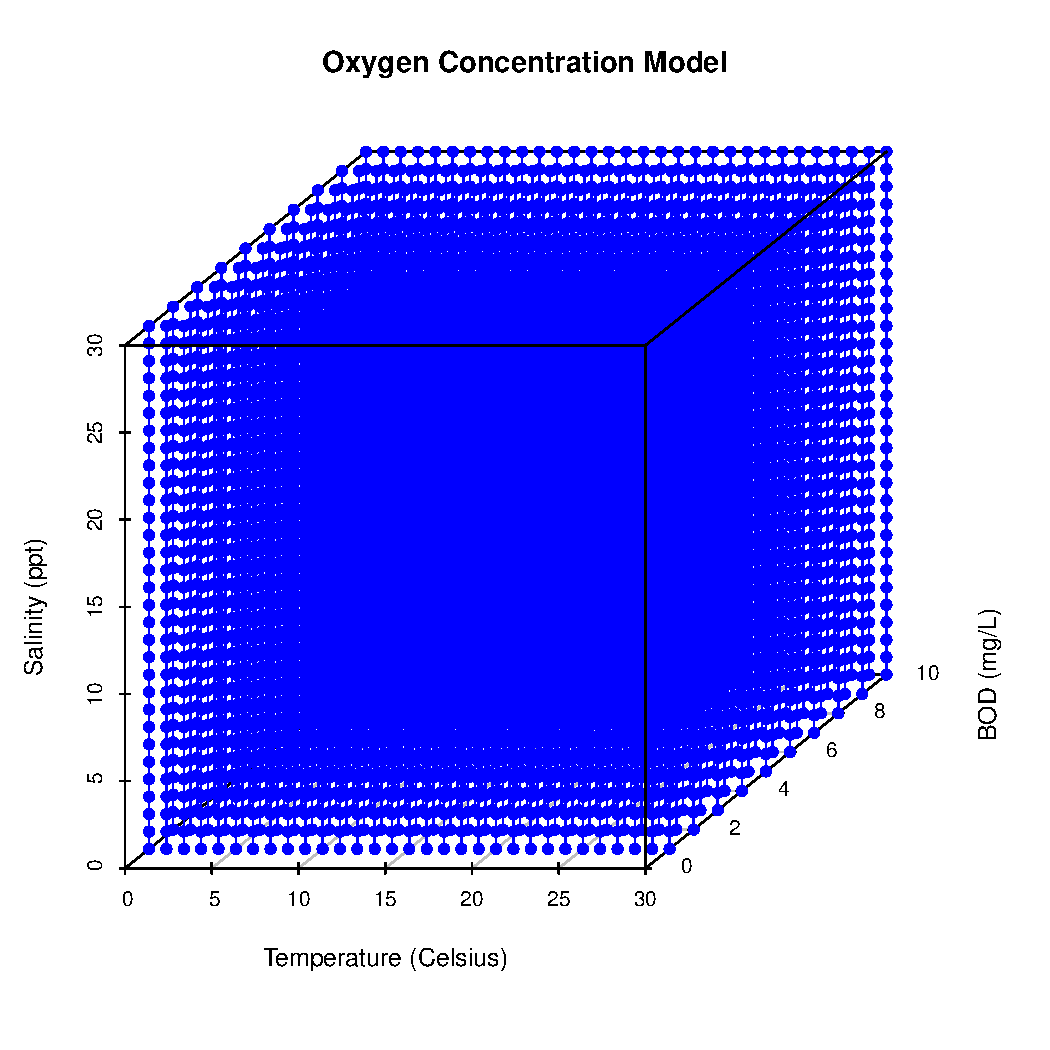
\includegraphics[width=\maxwidth]{figure/unnamed-chunk-1-1} 

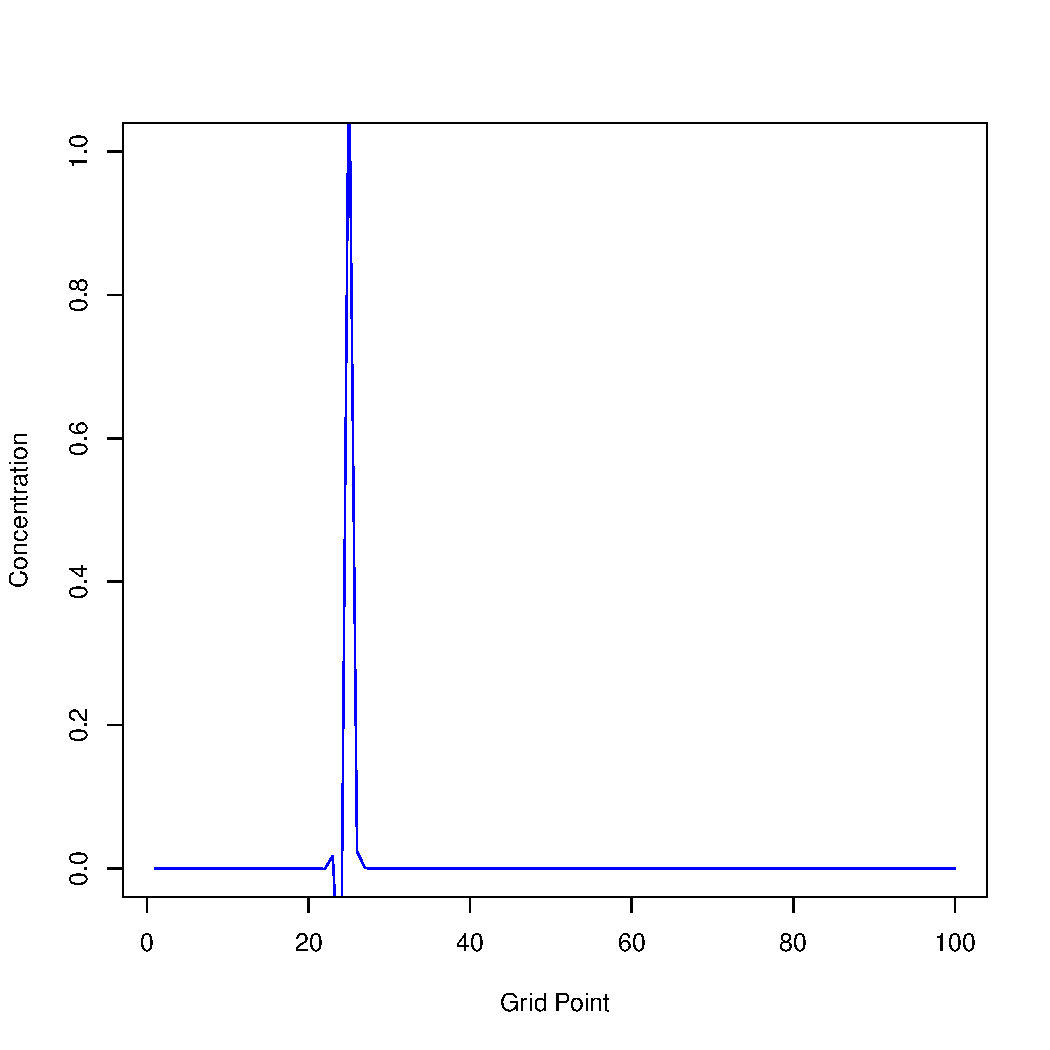
\includegraphics[width=\maxwidth]{figure/unnamed-chunk-1-2} 

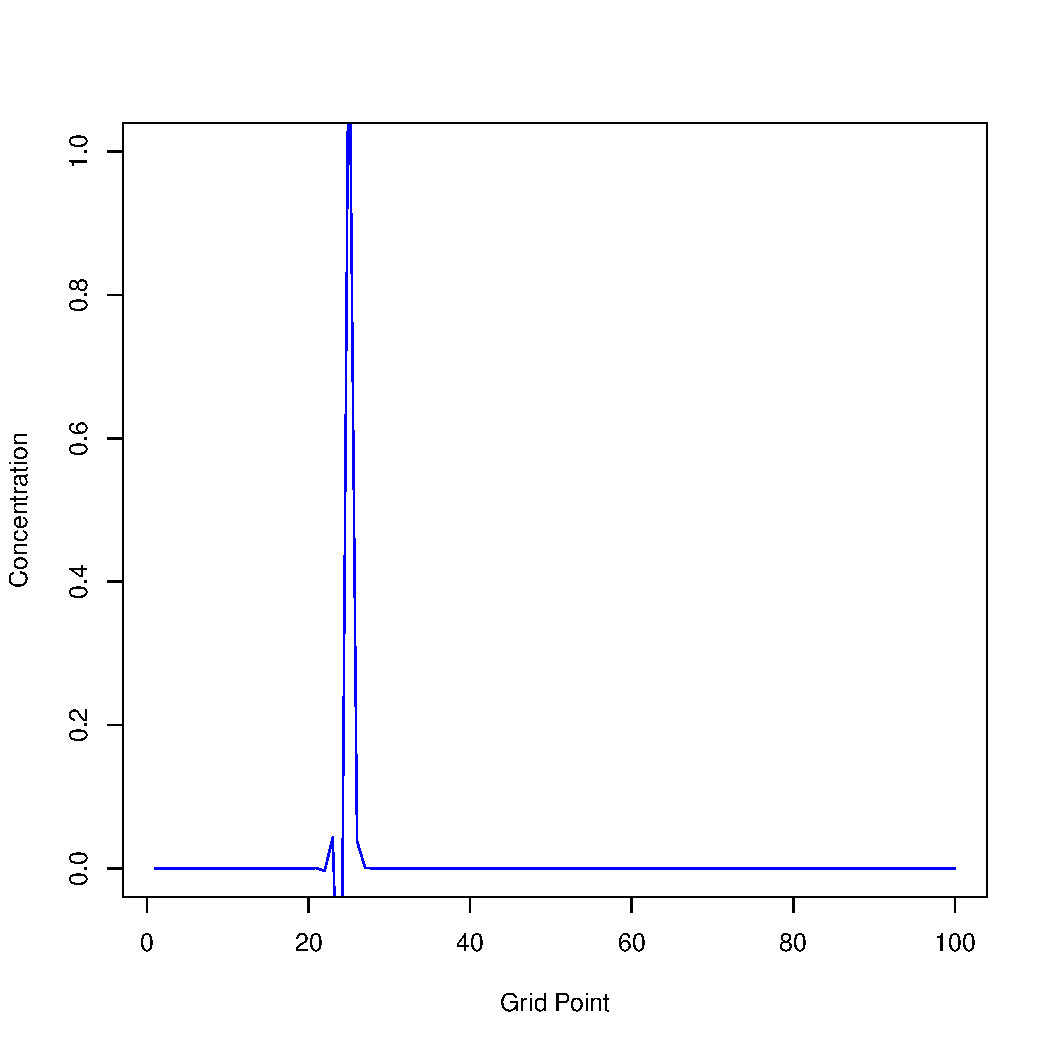
\includegraphics[width=\maxwidth]{figure/unnamed-chunk-1-3} 

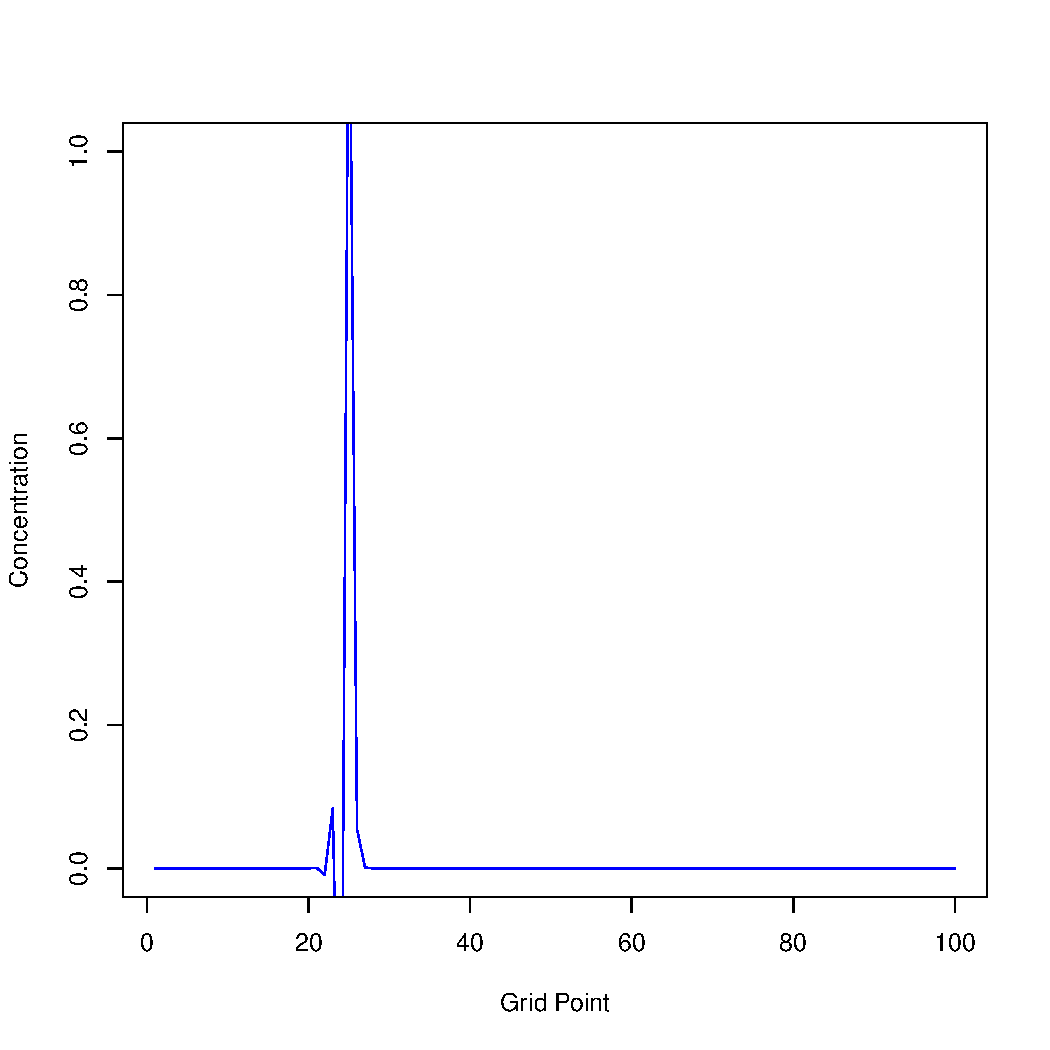
\includegraphics[width=\maxwidth]{figure/unnamed-chunk-1-4} 

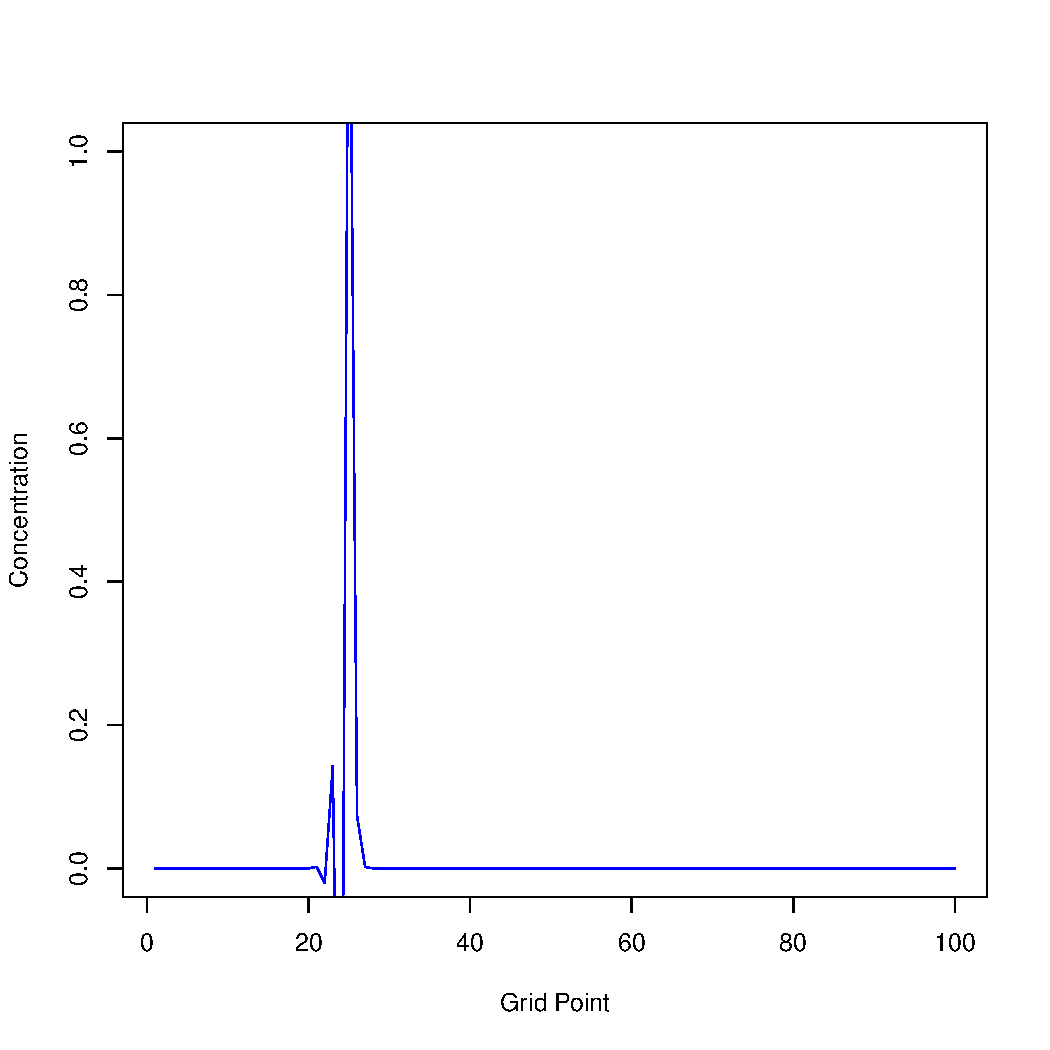
\includegraphics[width=\maxwidth]{figure/unnamed-chunk-1-5} 

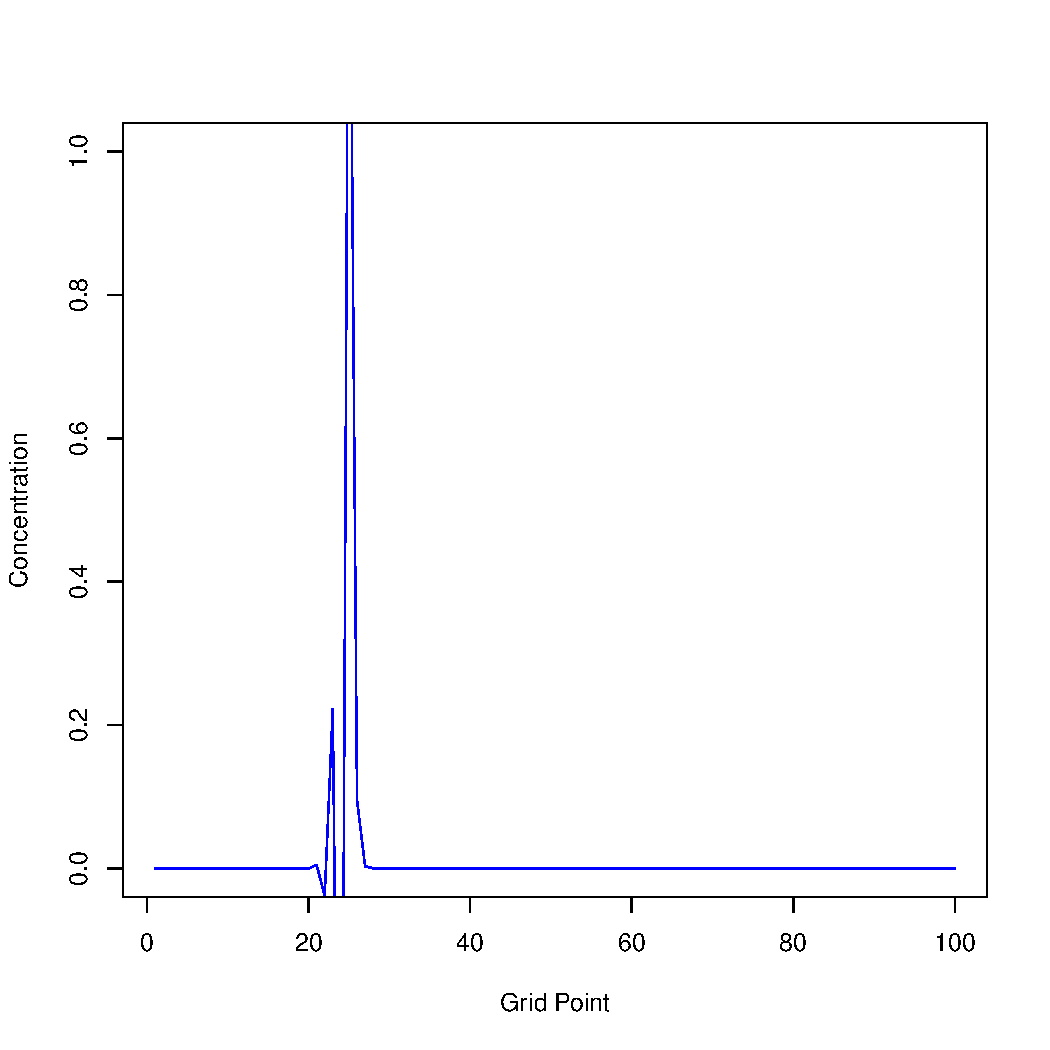
\includegraphics[width=\maxwidth]{figure/unnamed-chunk-1-6} 

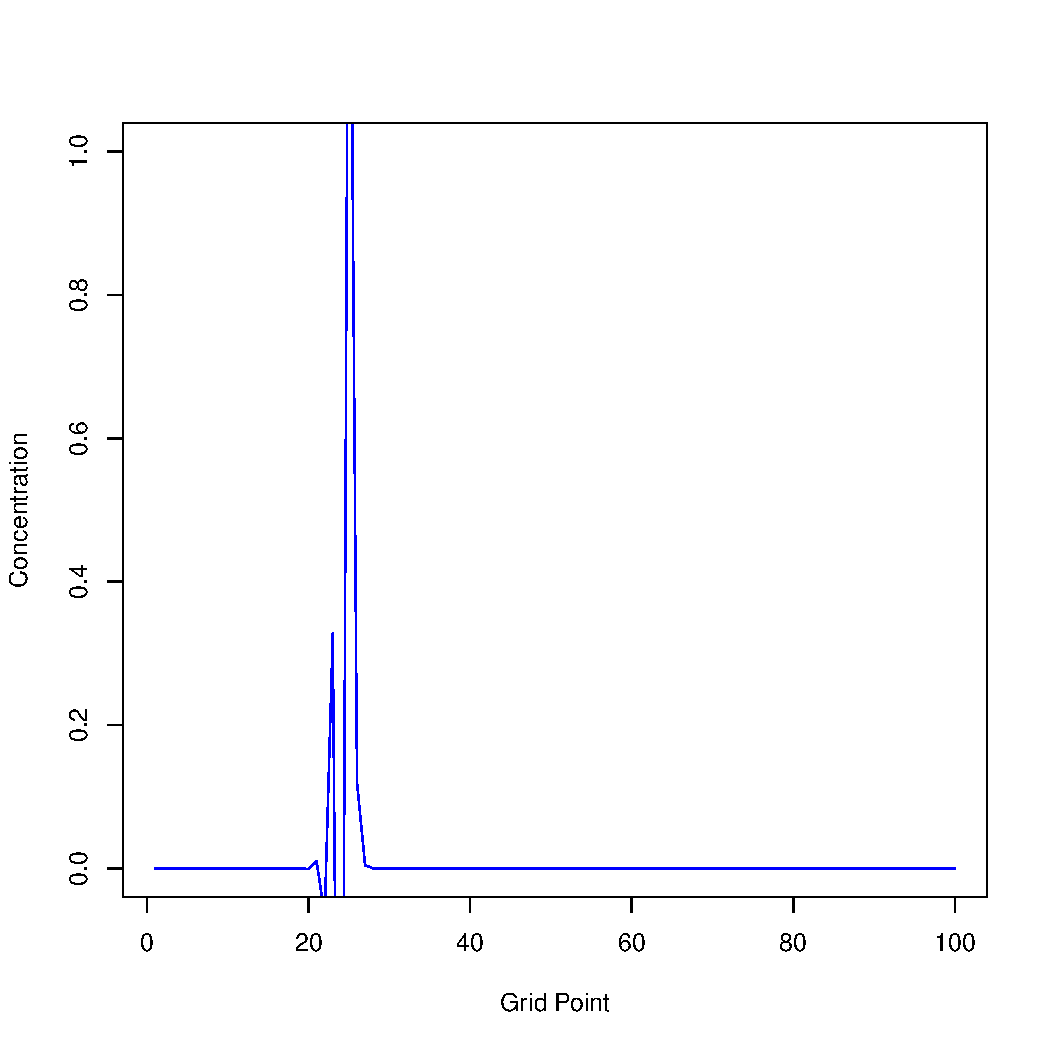
\includegraphics[width=\maxwidth]{figure/unnamed-chunk-1-7} 

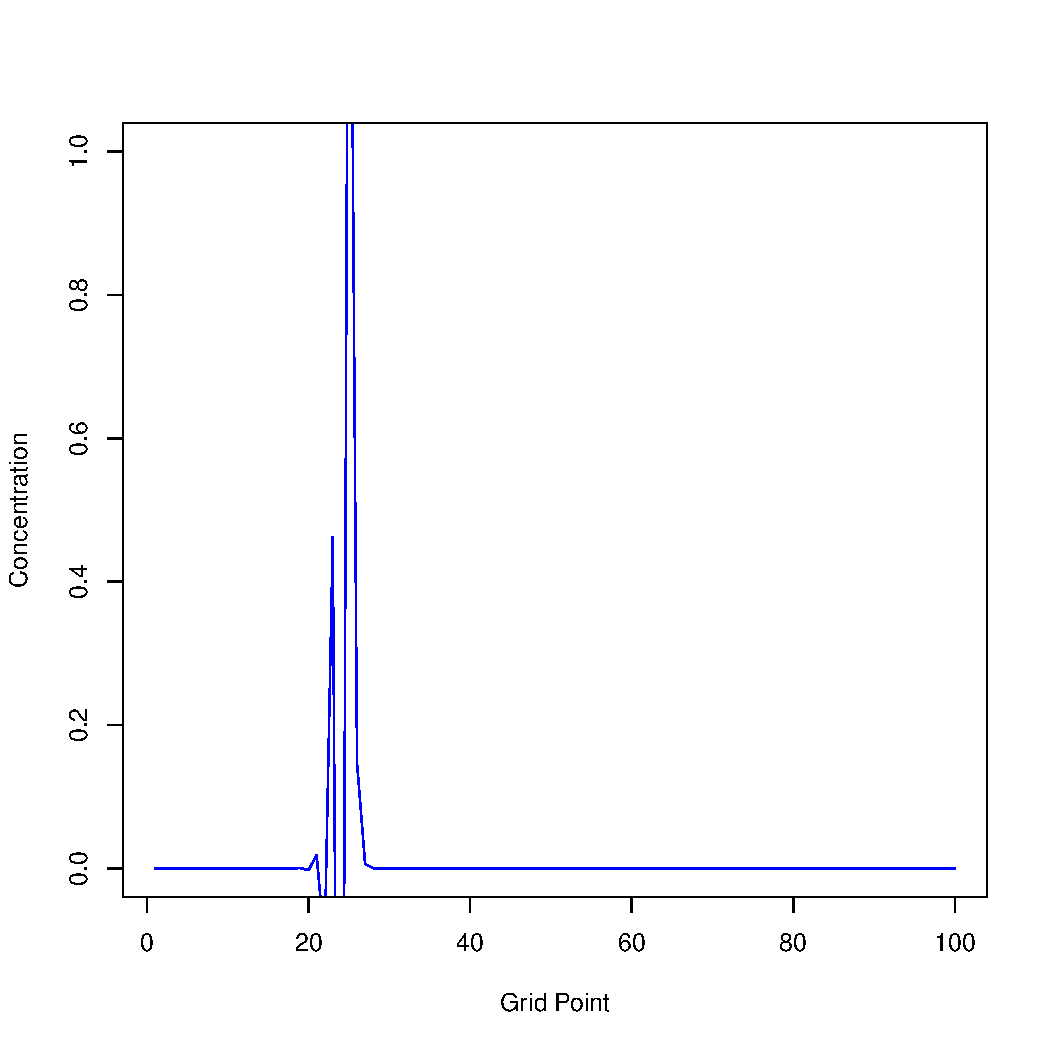
\includegraphics[width=\maxwidth]{figure/unnamed-chunk-1-8} 

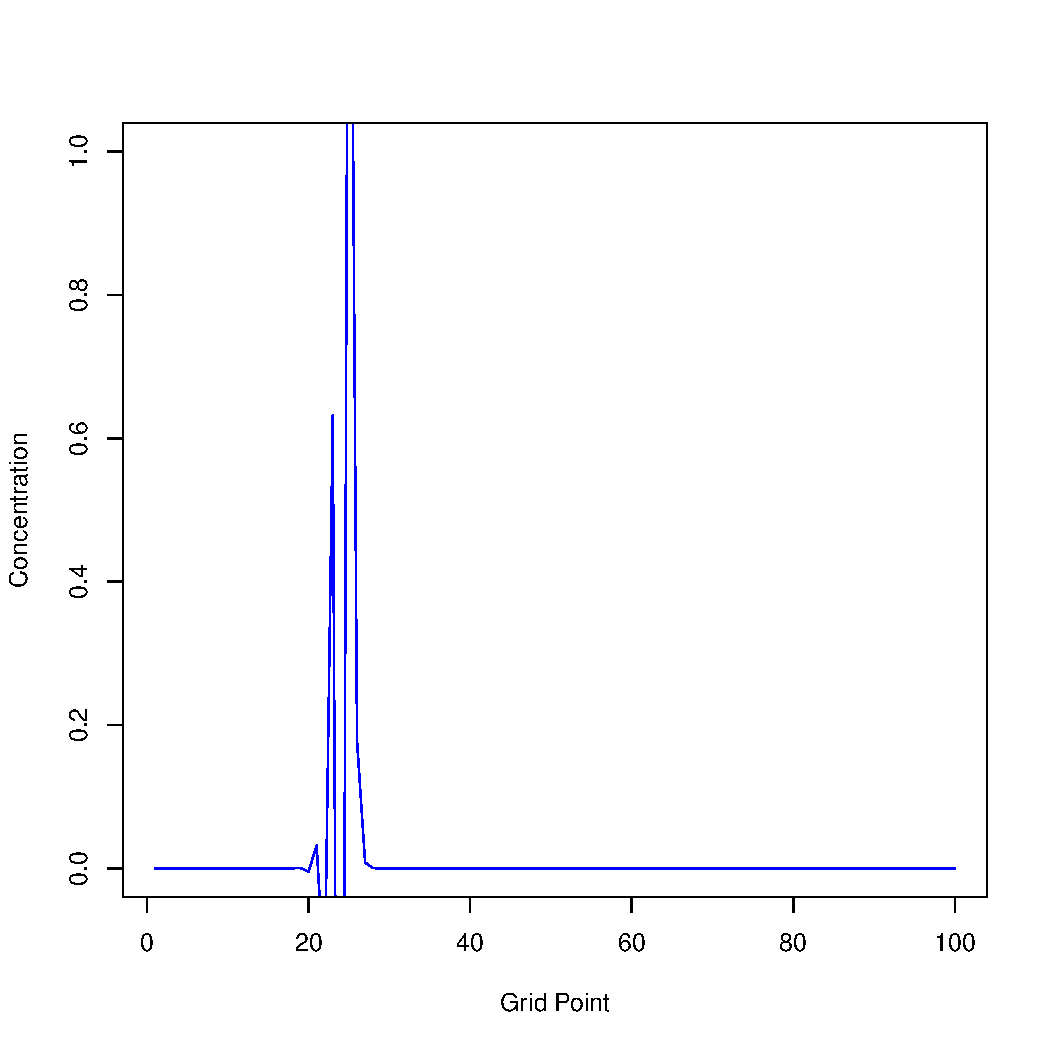
\includegraphics[width=\maxwidth]{figure/unnamed-chunk-1-9} 

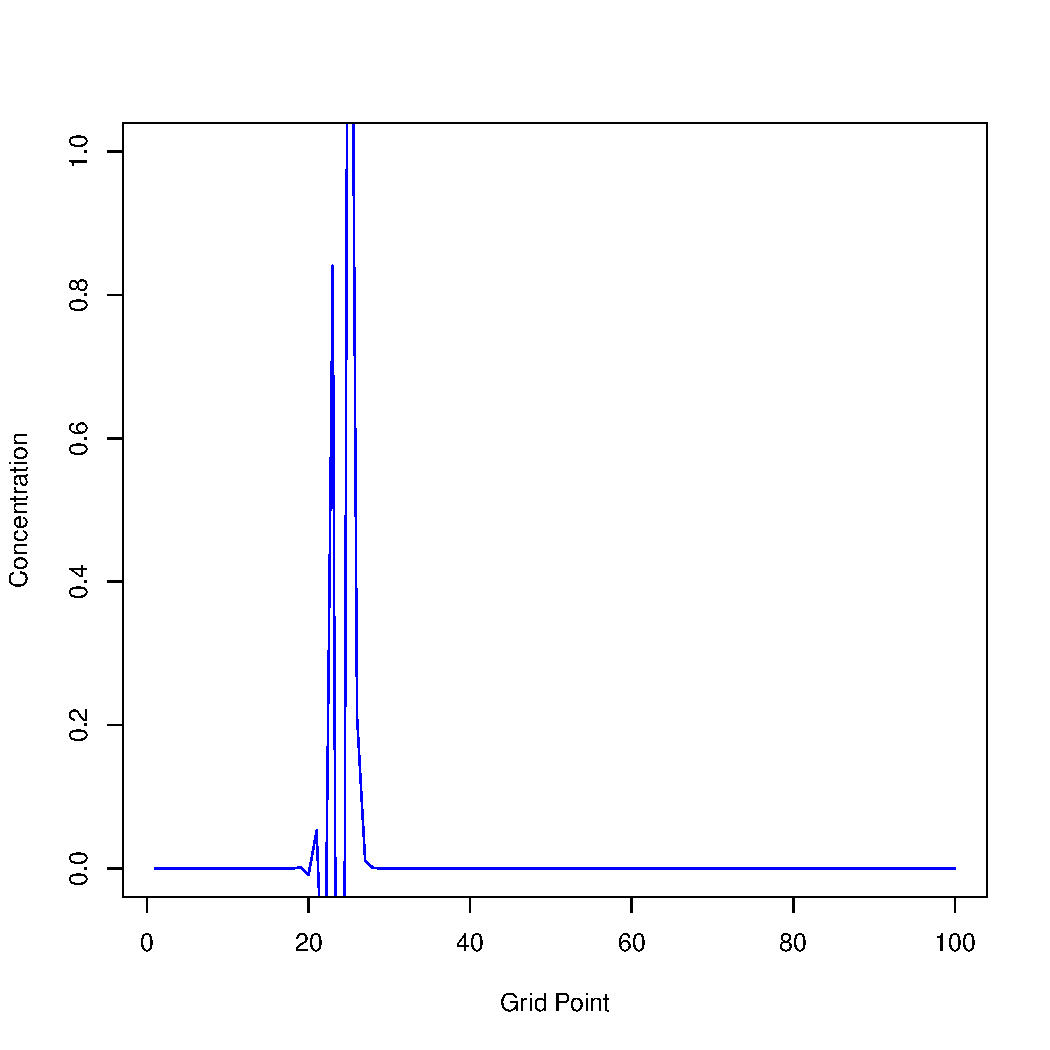
\includegraphics[width=\maxwidth]{figure/unnamed-chunk-1-10} 
\begin{kframe}\begin{alltt}
\hlcom{# Final plot}
\hlkwd{plot_grid}\hlstd{(grid)}
\end{alltt}
\end{kframe}
\end{knitrout}


\section{Modeling Advection and Diffusion}


\begin{knitrout}
\definecolor{shadecolor}{rgb}{0.969, 0.969, 0.969}\color{fgcolor}\begin{kframe}
\begin{alltt}
\hlcom{# Advection-Diffusion Modeling in R}

\hlcom{# Parameters}
\hlstd{L} \hlkwb{<-} \hlnum{10}          \hlcom{# Length of the domain}
\hlstd{T} \hlkwb{<-} \hlnum{1}           \hlcom{# Total simulation time}
\hlstd{Nx} \hlkwb{<-} \hlnum{100}         \hlcom{# Number of spatial grid points}
\hlstd{Nt} \hlkwb{<-} \hlnum{100}         \hlcom{# Number of time steps}
\hlstd{alpha} \hlkwb{<-} \hlnum{0.01}     \hlcom{# Diffusion coefficient}
\hlstd{beta} \hlkwb{<-} \hlnum{0.1}       \hlcom{# Advection coefficient}

\hlcom{# Discretization}
\hlstd{dx} \hlkwb{<-} \hlstd{L} \hlopt{/} \hlstd{(Nx} \hlopt{-} \hlnum{1}\hlstd{)}     \hlcom{# Spatial step size}
\hlstd{dt} \hlkwb{<-} \hlstd{T} \hlopt{/} \hlstd{Nt}           \hlcom{# Time step size}

\hlcom{# Initial conditions}
\hlstd{u} \hlkwb{<-} \hlkwd{rep}\hlstd{(}\hlnum{0}\hlstd{, Nx)}
\hlstd{u[Nx} \hlopt \hlnum{4}\hlopt{:}\hlstd{(}\hlnum{3} \hlopt{*} \hlstd{Nx} \hlopt \hlnum{4}\hlstd{)]} \hlkwb{<-} \hlnum{1}  \hlcom{# Initial pulse in the middle of the domain}

\hlcom{# Plot initial conditions}
\hlkwd{plot}\hlstd{(}\hlkwd{seq}\hlstd{(}\hlnum{0}\hlstd{, L,} \hlkwc{length.out} \hlstd{= Nx), u,} \hlkwc{type} \hlstd{=} \hlstr{"l"}\hlstd{,} \hlkwc{ylim} \hlstd{=} \hlkwd{c}\hlstd{(}\hlnum{0}\hlstd{,} \hlnum{1}\hlstd{),} \hlkwc{xlab} \hlstd{=} \hlstr{"Space"}\hlstd{,} \hlkwc{ylab} \hlstd{=} \hlstr{"Concentration"}\hlstd{,} \hlkwc{main} \hlstd{=} \hlstr{"Initial Conditions"}\hlstd{)}
\end{alltt}
\end{kframe}
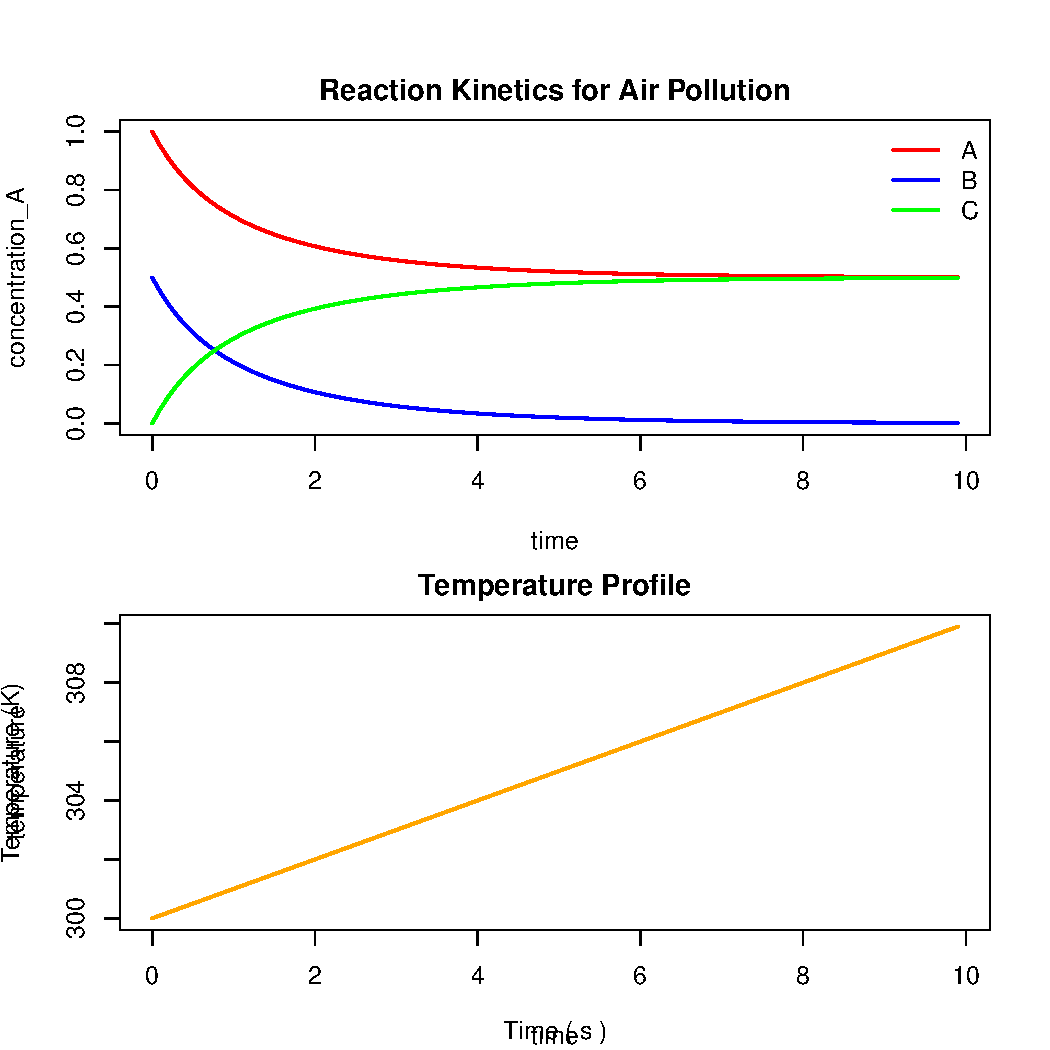
\includegraphics[width=\maxwidth]{figure/unnamed-chunk-2-1} 
\begin{kframe}\begin{alltt}
\hlcom{# Advection-Diffusion simulation using finite difference method}
\hlkwa{for} \hlstd{(t} \hlkwa{in} \hlnum{1}\hlopt{:}\hlstd{Nt) \{}
  \hlkwa{for} \hlstd{(x} \hlkwa{in} \hlnum{2}\hlopt{:}\hlstd{(Nx} \hlopt{-} \hlnum{1}\hlstd{)) \{}
    \hlstd{u[x]} \hlkwb{<-} \hlstd{u[x]} \hlopt{+} \hlstd{alpha} \hlopt{*} \hlstd{(u[x} \hlopt{+} \hlnum{1}\hlstd{]} \hlopt{-} \hlnum{2} \hlopt{*} \hlstd{u[x]} \hlopt{+} \hlstd{u[x} \hlopt{-} \hlnum{1}\hlstd{])} \hlopt{*} \hlstd{dt} \hlopt{/} \hlstd{dx}\hlopt{^}\hlnum{2} \hlopt{-} \hlstd{beta} \hlopt{*} \hlstd{(u[x} \hlopt{+} \hlnum{1}\hlstd{]} \hlopt{-} \hlstd{u[x} \hlopt{-} \hlnum{1}\hlstd{])} \hlopt{*} \hlstd{dt} \hlopt{/} \hlstd{(}\hlnum{2} \hlopt{*} \hlstd{dx)}
  \hlstd{\}}

  \hlcom{# Apply boundary conditions (zero-flux)}
  \hlstd{u[}\hlnum{1}\hlstd{]} \hlkwb{<-} \hlstd{u[}\hlnum{2}\hlstd{]}
  \hlstd{u[Nx]} \hlkwb{<-} \hlstd{u[Nx} \hlopt{-} \hlnum{1}\hlstd{]}

  \hlcom{# Plot the current state every 10 time steps}
  \hlkwa{if} \hlstd{(t} \hlopt \hlnum{10} \hlopt{==} \hlnum{0}\hlstd{) \{}
    \hlkwd{plot}\hlstd{(}\hlkwd{seq}\hlstd{(}\hlnum{0}\hlstd{, L,} \hlkwc{length.out} \hlstd{= Nx), u,} \hlkwc{type} \hlstd{=} \hlstr{"l"}\hlstd{,} \hlkwc{ylim} \hlstd{=} \hlkwd{c}\hlstd{(}\hlnum{0}\hlstd{,} \hlnum{1}\hlstd{),} \hlkwc{xlab} \hlstd{=} \hlstr{"Space"}\hlstd{,} \hlkwc{ylab} \hlstd{=} \hlstr{"Concentration"}\hlstd{,} \hlkwc{main} \hlstd{=} \hlkwd{paste}\hlstd{(}\hlstr{"Time ="}\hlstd{, t} \hlopt{*} \hlstd{dt))}
    \hlkwd{Sys.sleep}\hlstd{(}\hlnum{0.1}\hlstd{)}  \hlcom{# Pause to visualize the animation}
  \hlstd{\}}
\hlstd{\}}
\end{alltt}
\end{kframe}
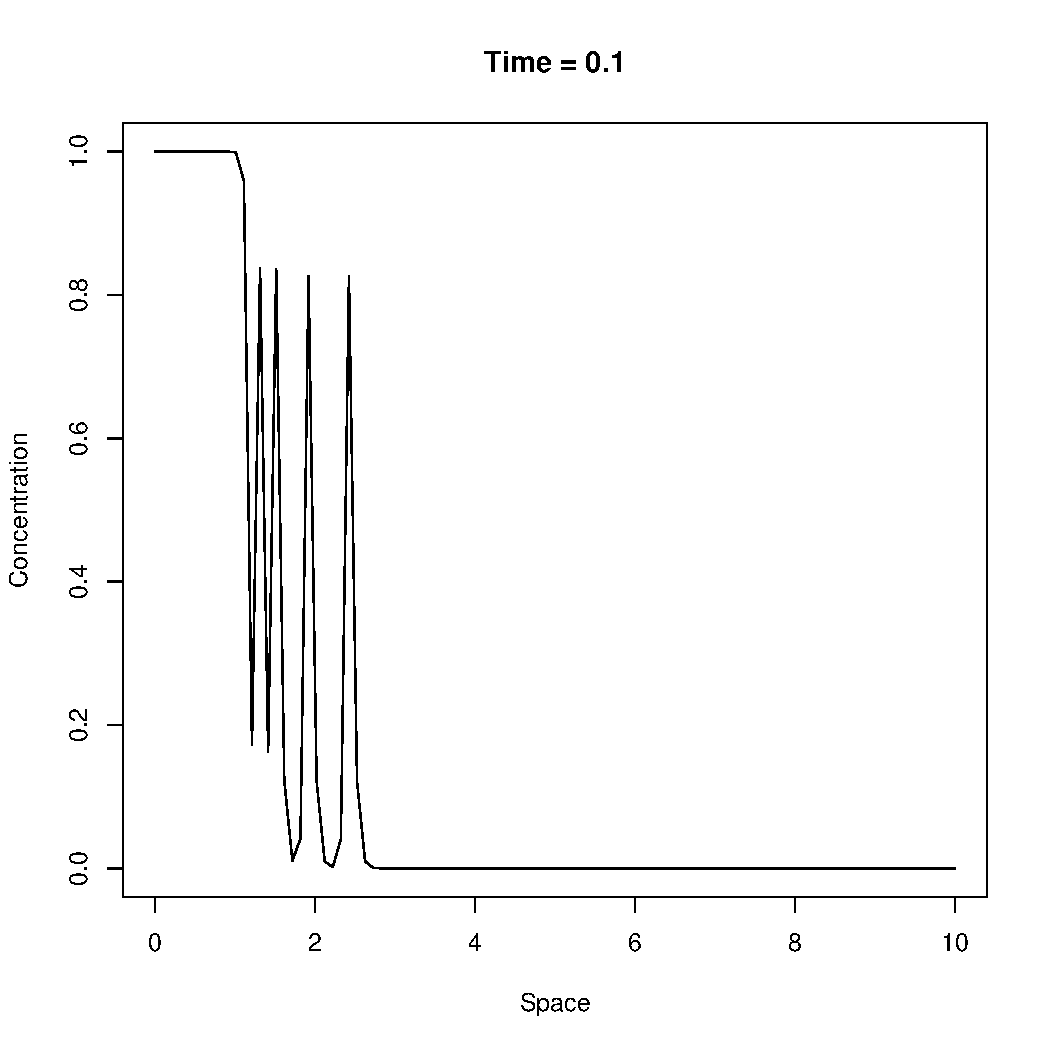
\includegraphics[width=\maxwidth]{figure/unnamed-chunk-2-2} 

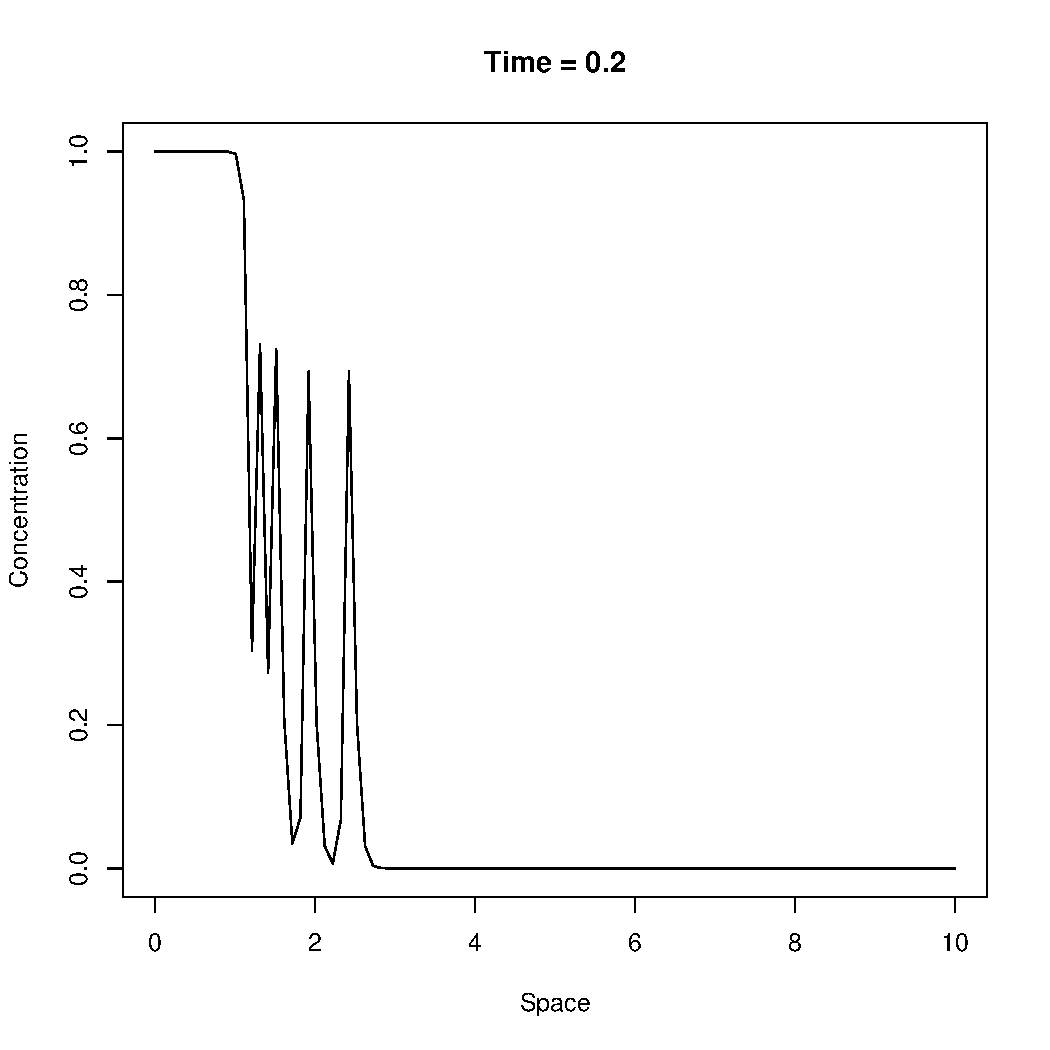
\includegraphics[width=\maxwidth]{figure/unnamed-chunk-2-3} 

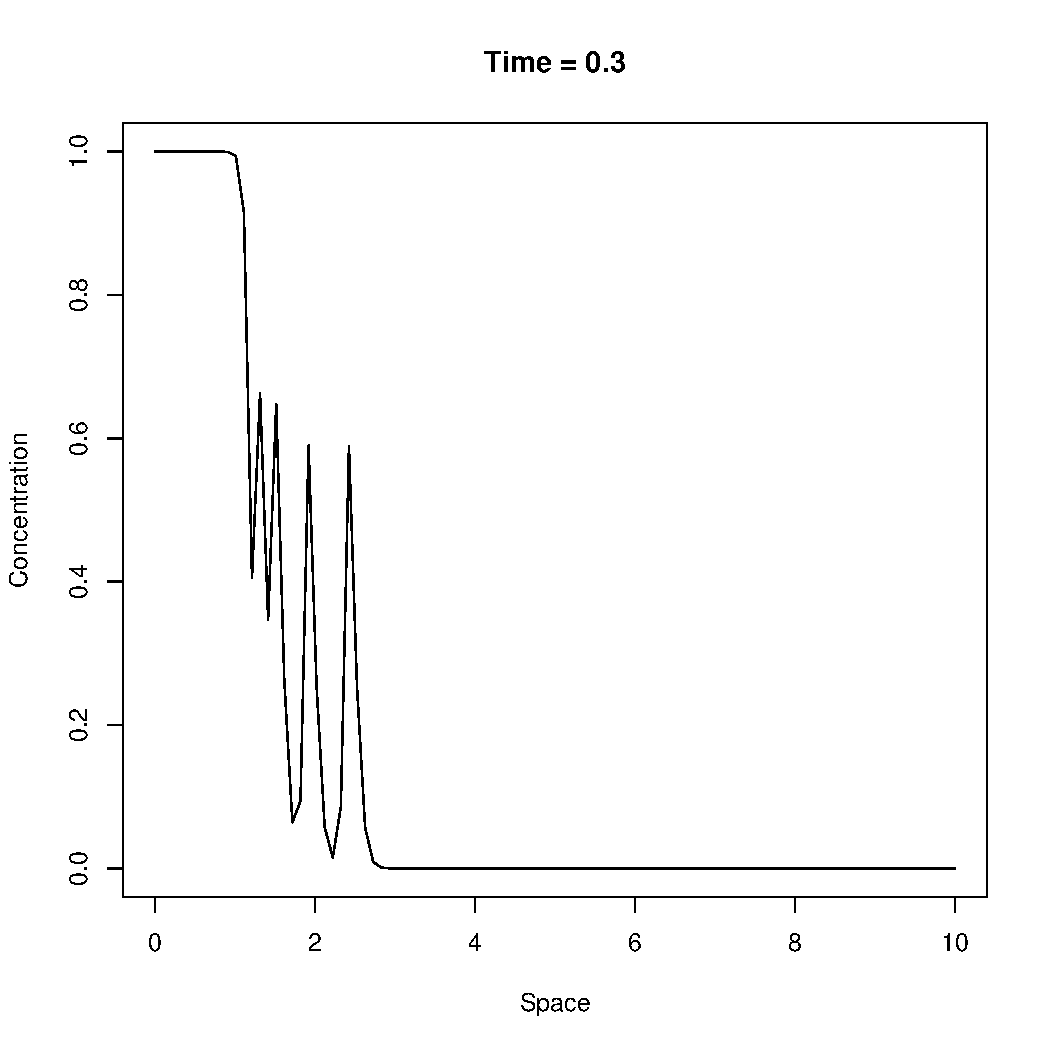
\includegraphics[width=\maxwidth]{figure/unnamed-chunk-2-4} 

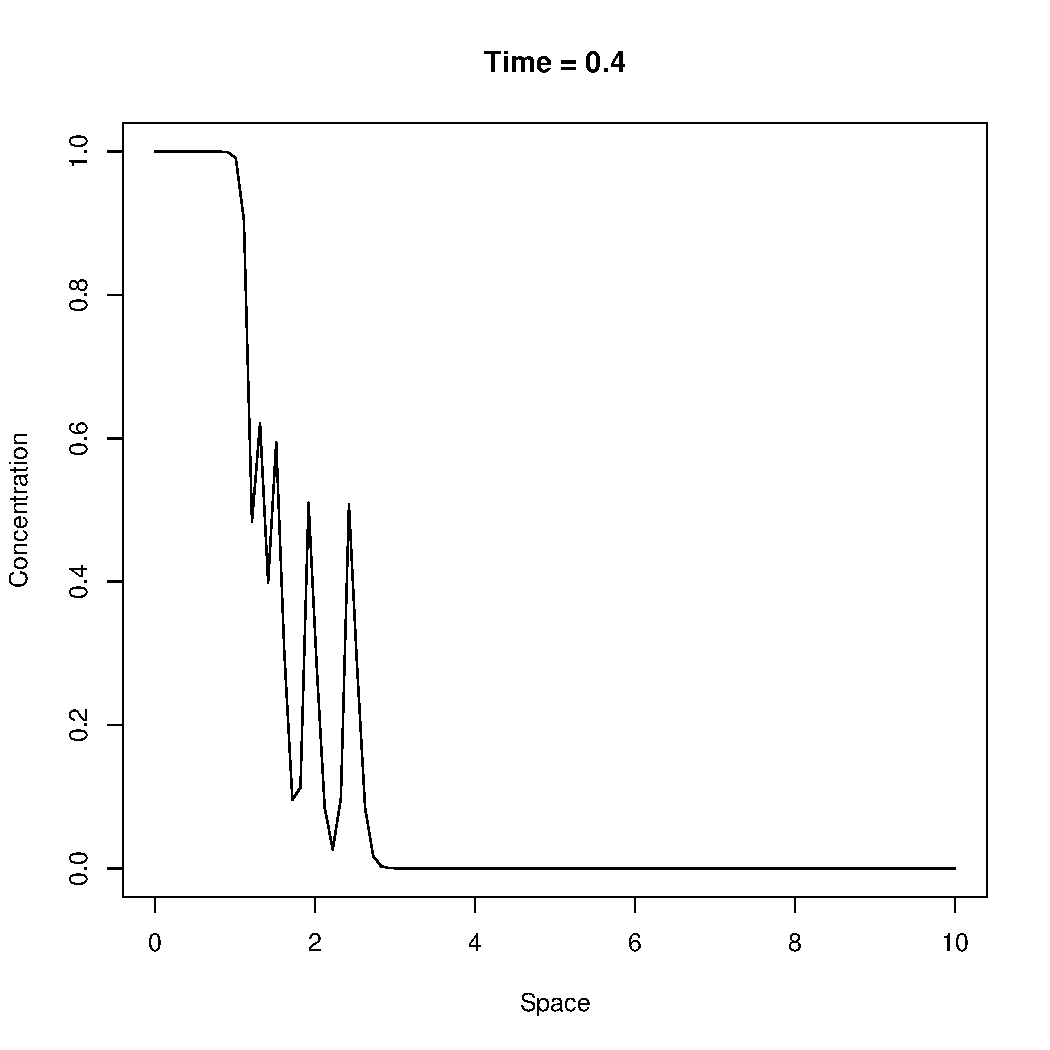
\includegraphics[width=\maxwidth]{figure/unnamed-chunk-2-5} 

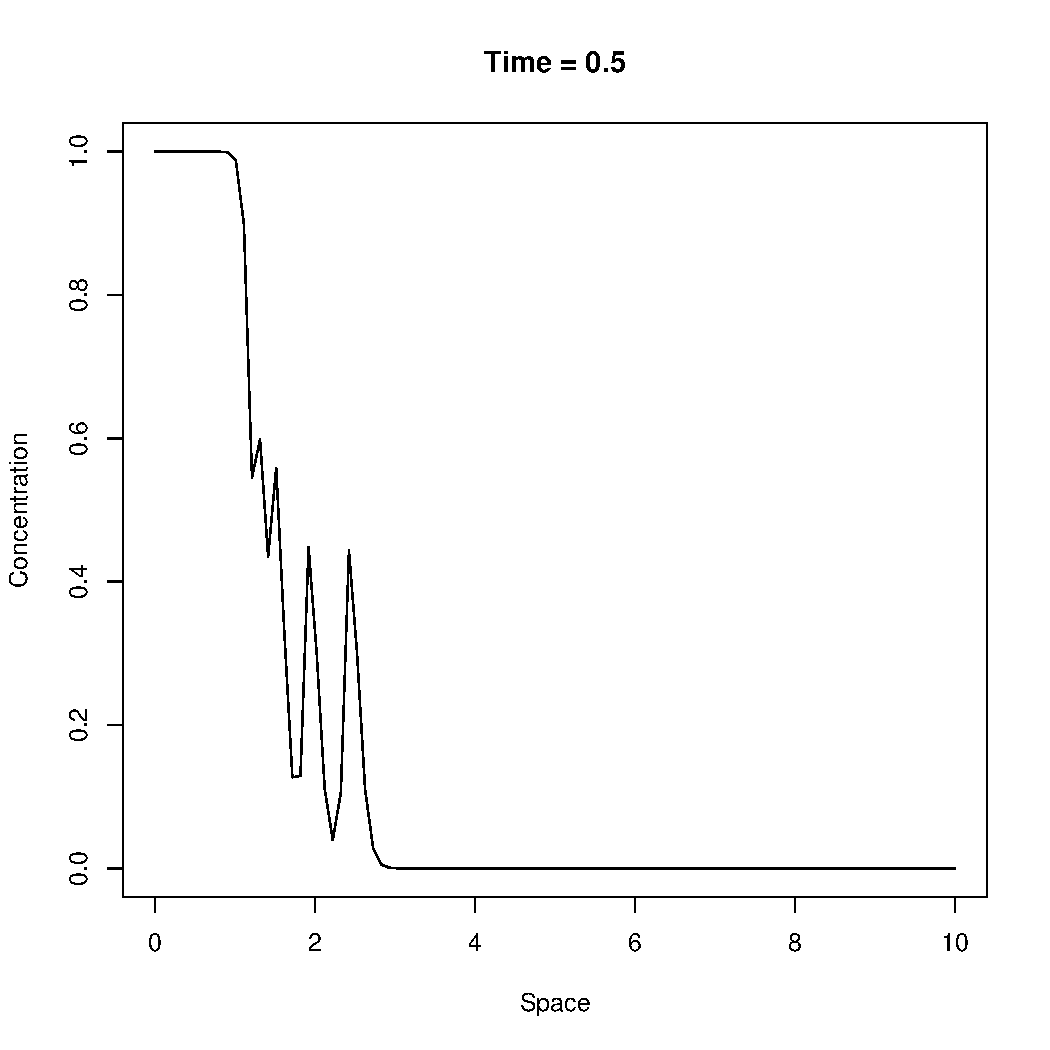
\includegraphics[width=\maxwidth]{figure/unnamed-chunk-2-6} 

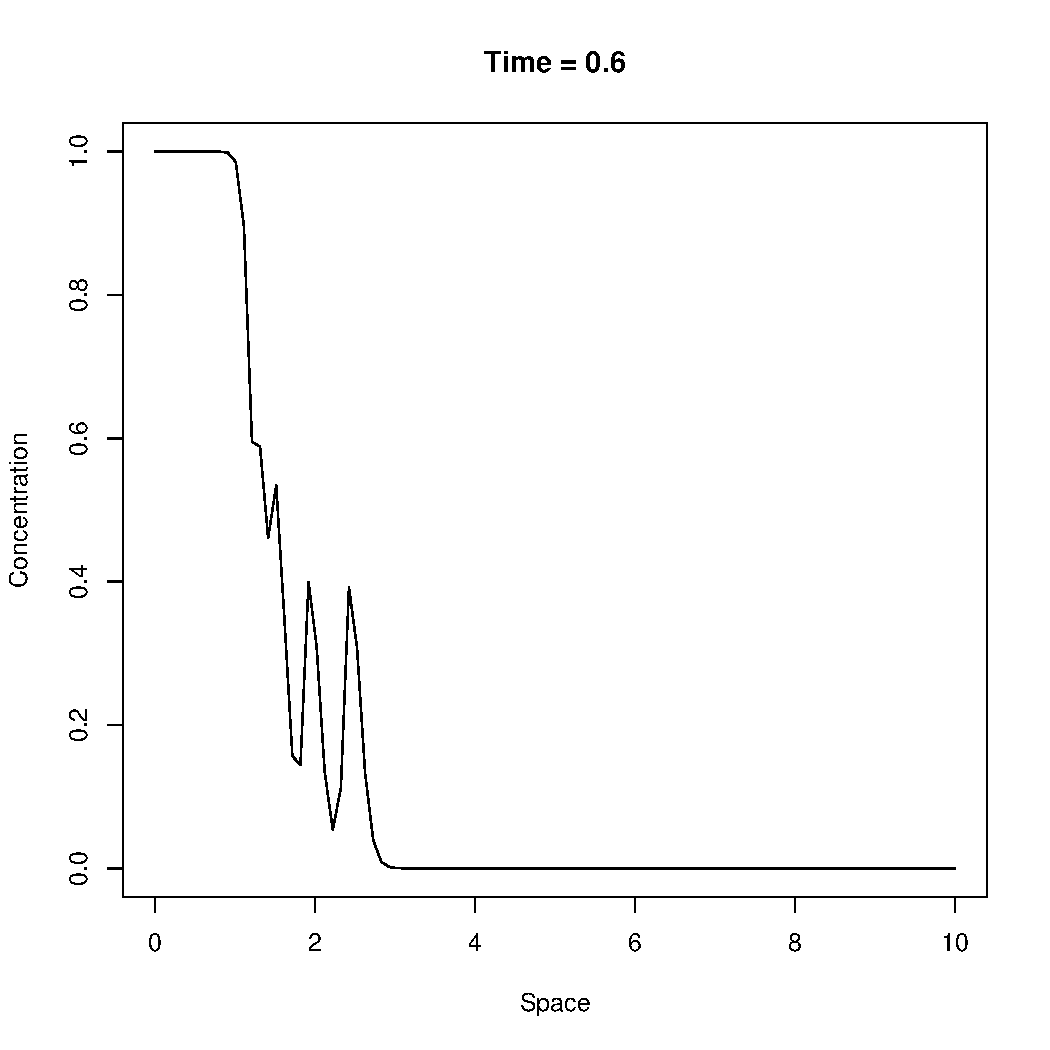
\includegraphics[width=\maxwidth]{figure/unnamed-chunk-2-7} 

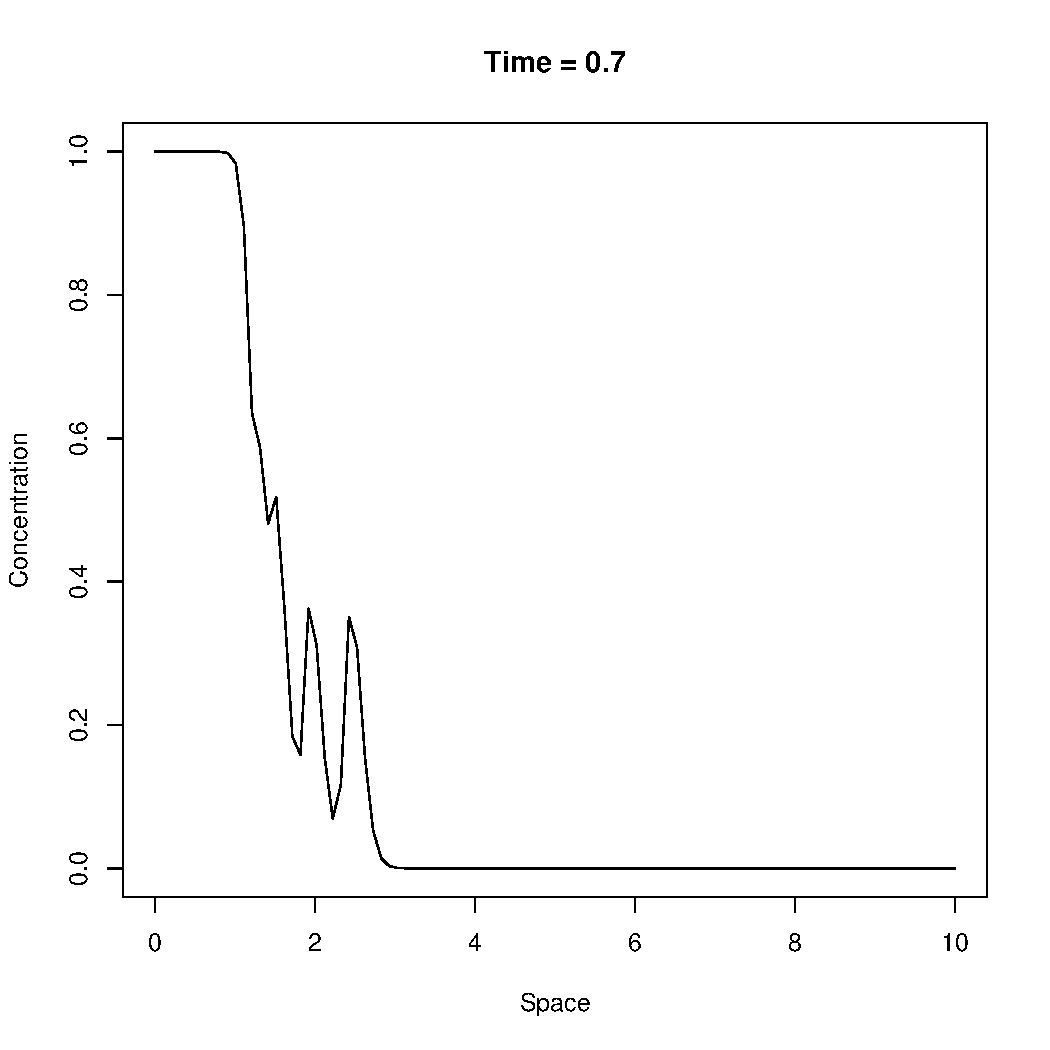
\includegraphics[width=\maxwidth]{figure/unnamed-chunk-2-8} 

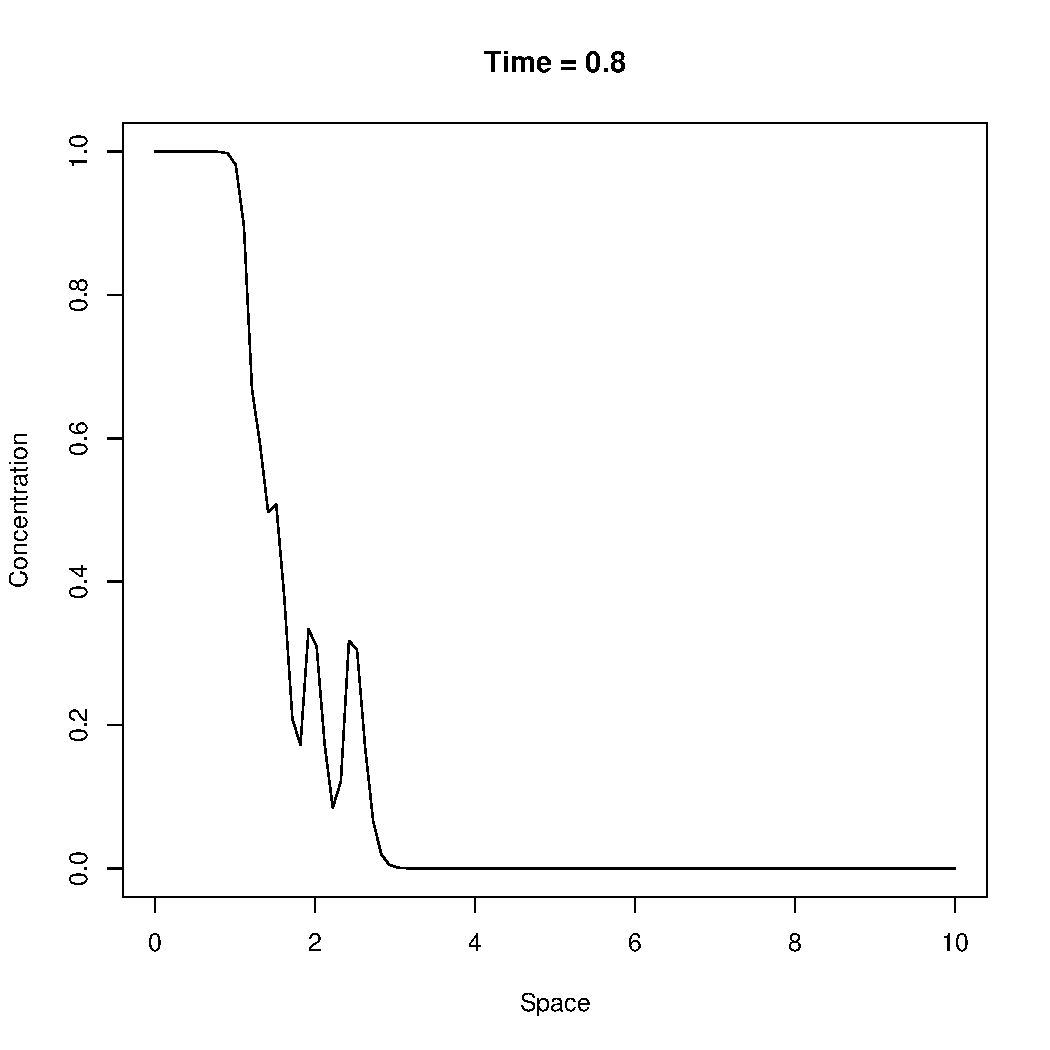
\includegraphics[width=\maxwidth]{figure/unnamed-chunk-2-9} 

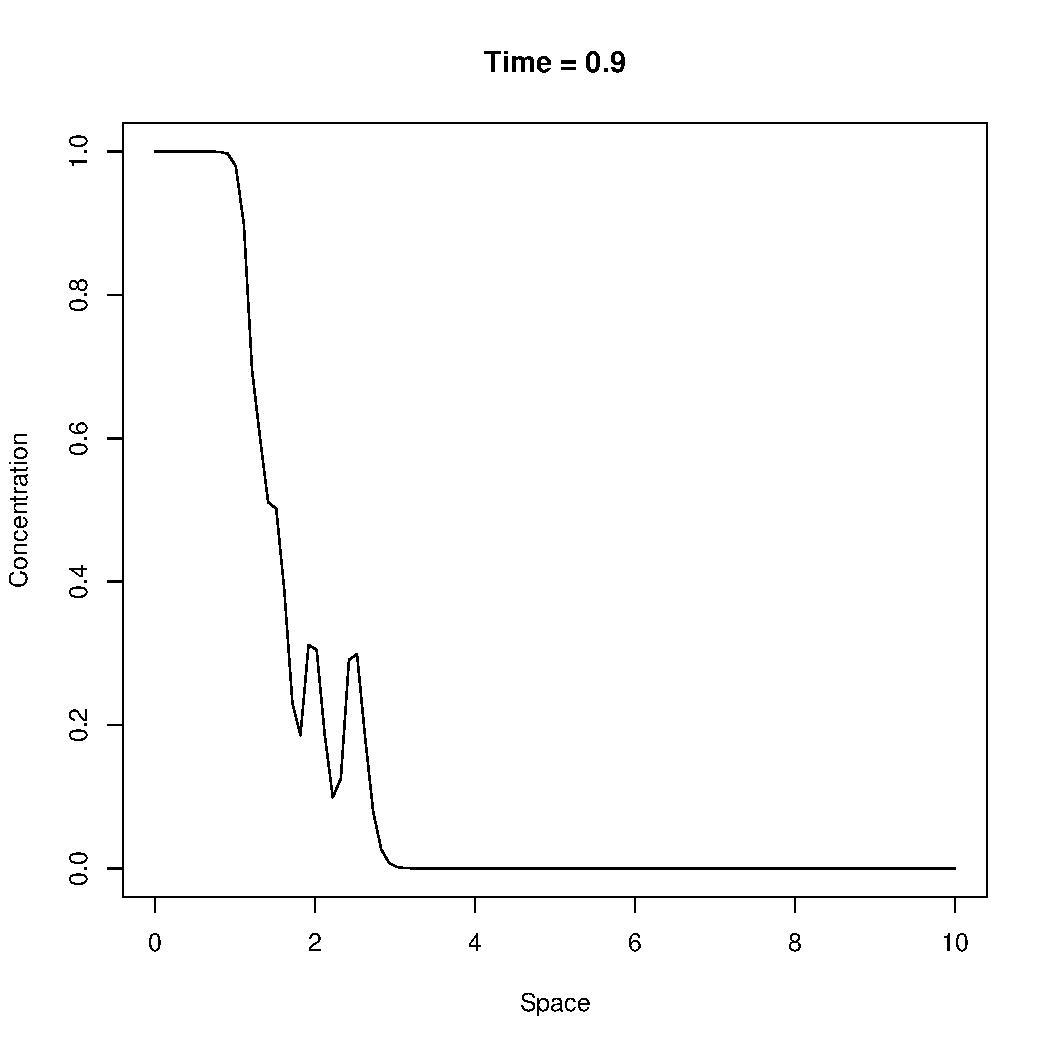
\includegraphics[width=\maxwidth]{figure/unnamed-chunk-2-10} 

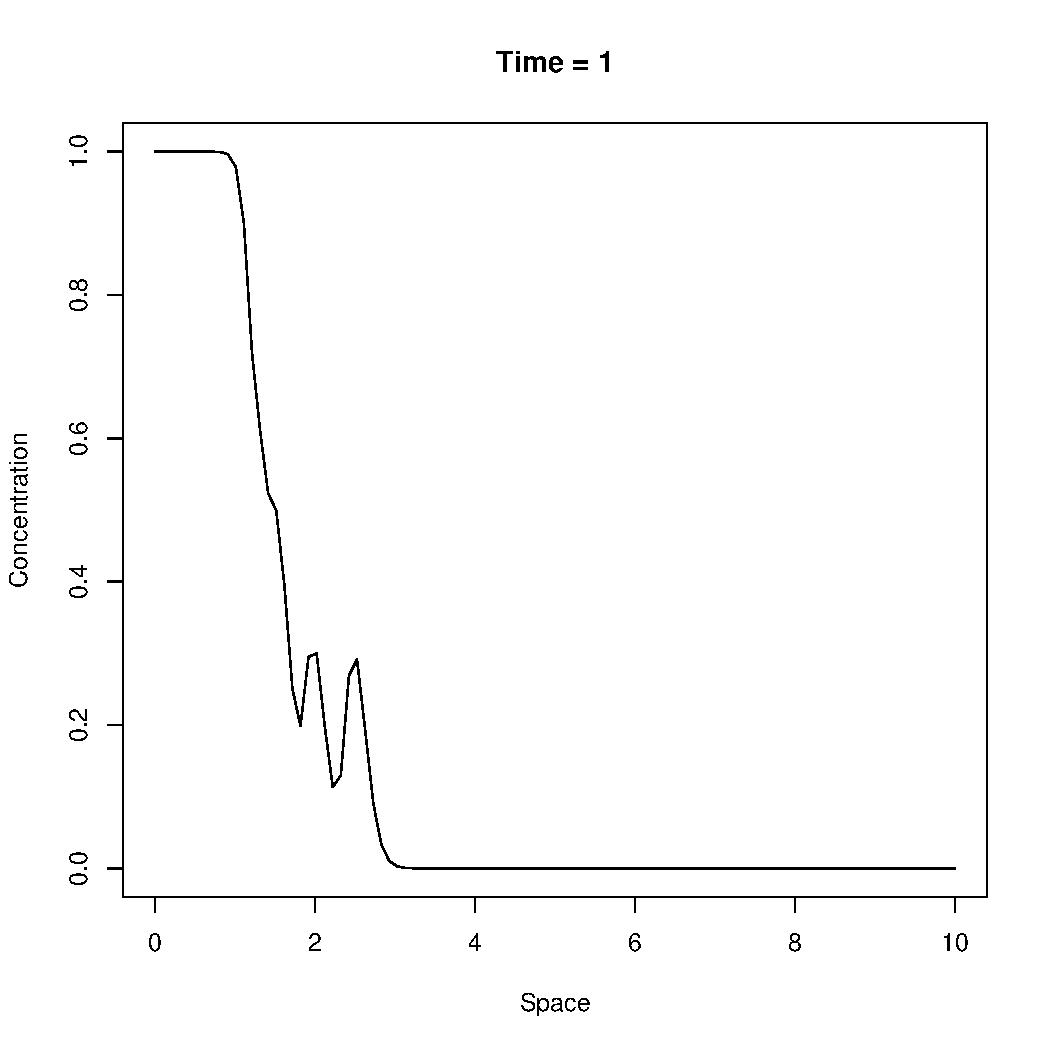
\includegraphics[width=\maxwidth]{figure/unnamed-chunk-2-11} 
\begin{kframe}\begin{alltt}
\hlcom{# Plot the final state}
\hlkwd{plot}\hlstd{(}\hlkwd{seq}\hlstd{(}\hlnum{0}\hlstd{, L,} \hlkwc{length.out} \hlstd{= Nx), u,} \hlkwc{type} \hlstd{=} \hlstr{"l"}\hlstd{,} \hlkwc{ylim} \hlstd{=} \hlkwd{c}\hlstd{(}\hlnum{0}\hlstd{,} \hlnum{1}\hlstd{),} \hlkwc{xlab} \hlstd{=} \hlstr{"Space"}\hlstd{,} \hlkwc{ylab} \hlstd{=} \hlstr{"Concentration"}\hlstd{,} \hlkwc{main} \hlstd{=} \hlstr{"Final State"}\hlstd{)}
\end{alltt}
\end{kframe}
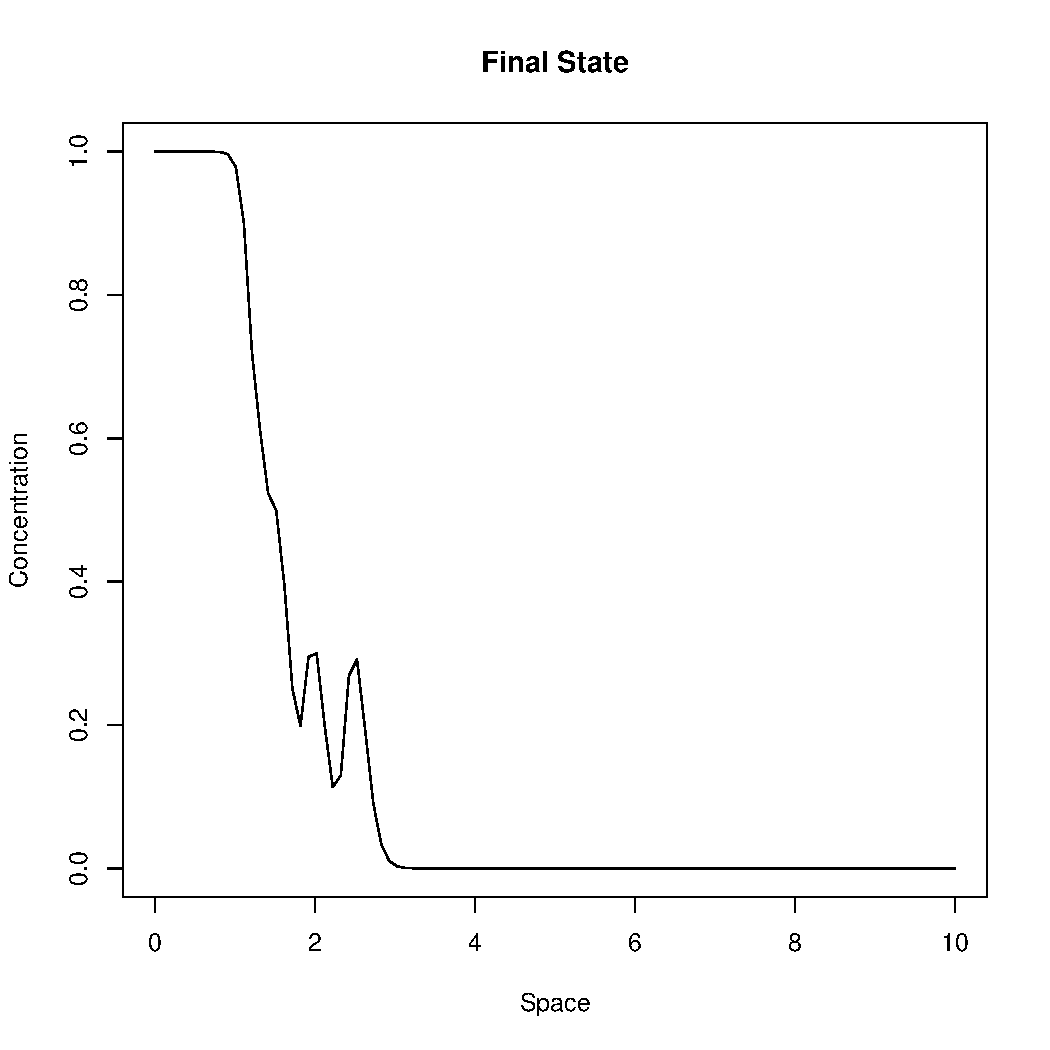
\includegraphics[width=\maxwidth]{figure/unnamed-chunk-2-12} 
\end{knitrout}

This code sets up a simple 1D advection-diffusion simulation with a pulse as the initial condition. The finite difference method is used to update the concentration at each spatial point over time. The simulation progresses in time steps, and the final state is plotted. You can adjust the parameters (e.g., diffusion coefficient, advection coefficient, grid size, time steps) to see how they affect the simulation.

\section{Modeling Advection and Diffusion}

Below is an example of R code for simulating advection and diffusion using a simple finite difference method. This code assumes a one-dimensional domain for simplicity.

\begin{knitrout}
\definecolor{shadecolor}{rgb}{0.969, 0.969, 0.969}\color{fgcolor}\begin{kframe}
\begin{alltt}
\hlcom{# Advection-Diffusion Modeling in R}

\hlcom{# Parameters}
\hlstd{length_domain} \hlkwb{<-} \hlnum{10}  \hlcom{# Length of the domain}
\hlstd{num_points} \hlkwb{<-} \hlnum{100}    \hlcom{# Number of spatial points}
\hlstd{dx} \hlkwb{<-} \hlstd{length_domain} \hlopt{/} \hlstd{(num_points} \hlopt{-} \hlnum{1}\hlstd{)}  \hlcom{# Spatial grid size}
\hlstd{dt} \hlkwb{<-} \hlnum{0.1}            \hlcom{# Time step}
\hlstd{num_steps} \hlkwb{<-} \hlnum{100}     \hlcom{# Number of time steps}

\hlcom{# Advection and diffusion coefficients}
\hlstd{velocity} \hlkwb{<-} \hlnum{0.5}      \hlcom{# Advection velocity}
\hlstd{diffusion_coeff} \hlkwb{<-} \hlnum{0.01}  \hlcom{# Diffusion coefficient}

\hlcom{# Initial condition}
\hlstd{initial_condition} \hlkwb{<-} \hlkwa{function}\hlstd{(}\hlkwc{x}\hlstd{) \{}
  \hlkwd{return}\hlstd{(}\hlkwd{exp}\hlstd{(}\hlopt{-}\hlstd{((x} \hlopt{-} \hlstd{length_domain}\hlopt{/}\hlnum{4}\hlstd{)}\hlopt{^}\hlnum{2}\hlstd{)}\hlopt{/}\hlstd{(}\hlnum{2}\hlopt{*}\hlnum{1}\hlopt{^}\hlnum{2}\hlstd{)))}
\hlstd{\}}

\hlcom{# Initialize the concentration field}
\hlstd{concentration} \hlkwb{<-} \hlkwd{initial_condition}\hlstd{(}\hlkwd{seq}\hlstd{(}\hlnum{0}\hlstd{, length_domain,} \hlkwc{by} \hlstd{= dx))}

\hlcom{# Plot initial condition}
\hlkwd{plot}\hlstd{(}\hlkwd{seq}\hlstd{(}\hlnum{0}\hlstd{, length_domain,} \hlkwc{by} \hlstd{= dx), concentration,} \hlkwc{type} \hlstd{=} \hlstr{'l'}\hlstd{,} \hlkwc{col} \hlstd{=} \hlstr{'blue'}\hlstd{,}
     \hlkwc{ylim} \hlstd{=} \hlkwd{c}\hlstd{(}\hlnum{0}\hlstd{,} \hlnum{1}\hlstd{),} \hlkwc{main} \hlstd{=} \hlstr{'Advection-Diffusion Simulation'}\hlstd{,}
     \hlkwc{xlab} \hlstd{=} \hlstr{'Spatial Coordinate'}\hlstd{,} \hlkwc{ylab} \hlstd{=} \hlstr{'Concentration'}\hlstd{)}

\hlcom{# Simulation loop}
\hlkwa{for} \hlstd{(step} \hlkwa{in} \hlnum{1}\hlopt{:}\hlstd{num_steps) \{}
  \hlcom{# Advection term}
  \hlstd{advected_concentration} \hlkwb{<-} \hlkwd{c}\hlstd{(concentration[}\hlopt{-}\hlnum{1}\hlstd{], concentration[}\hlnum{1}\hlstd{])}

  \hlcom{# Diffusion term}
  \hlstd{diffused_concentration} \hlkwb{<-} \hlstd{diffusion_coeff} \hlopt{*} \hlstd{(}\hlkwd{c}\hlstd{(concentration[}\hlnum{2}\hlopt{:}\hlstd{num_points], concentration[num_points])} \hlopt{-} \hlnum{2} \hlopt{*} \hlstd{concentration} \hlopt{+} \hlkwd{c}\hlstd{(concentration[}\hlnum{1}\hlstd{], concentration[}\hlnum{1}\hlopt{:}\hlstd{(num_points}\hlopt{-}\hlnum{1}\hlstd{)]))} \hlopt{/} \hlstd{dx}\hlopt{^}\hlnum{2}

  \hlcom{# Update concentration using finite difference method}
  \hlstd{concentration} \hlkwb{<-} \hlstd{concentration} \hlopt{-} \hlstd{velocity} \hlopt{*} \hlstd{(advected_concentration} \hlopt{-} \hlstd{concentration)} \hlopt{*} \hlstd{dt} \hlopt{/} \hlstd{dx} \hlopt{+} \hlstd{diffused_concentration} \hlopt{*} \hlstd{dt}

  \hlcom{# Plot the updated concentration}
  \hlkwd{lines}\hlstd{(}\hlkwd{seq}\hlstd{(}\hlnum{0}\hlstd{, length_domain,} \hlkwc{by} \hlstd{= dx), concentration,} \hlkwc{col} \hlstd{=} \hlkwd{rgb}\hlstd{(}\hlnum{0}\hlstd{,} \hlnum{0}\hlstd{, step}\hlopt{/}\hlstd{num_steps),} \hlkwc{lwd} \hlstd{=} \hlnum{2}\hlstd{)}
\hlstd{\}}

\hlcom{# Add a legend}
\hlkwd{legend}\hlstd{(}\hlstr{'topright'}\hlstd{,} \hlkwc{legend} \hlstd{=} \hlkwd{paste}\hlstd{(}\hlstr{'Step'}\hlstd{,} \hlnum{1}\hlopt{:}\hlstd{num_steps),} \hlkwc{col} \hlstd{=} \hlkwd{rgb}\hlstd{(}\hlnum{0}\hlstd{,} \hlnum{0}\hlstd{,} \hlnum{1}\hlopt{:}\hlstd{num_steps,} \hlkwc{maxColorValue} \hlstd{= num_steps),} \hlkwc{lwd} \hlstd{=} \hlnum{2}\hlstd{)}
\end{alltt}
\end{kframe}
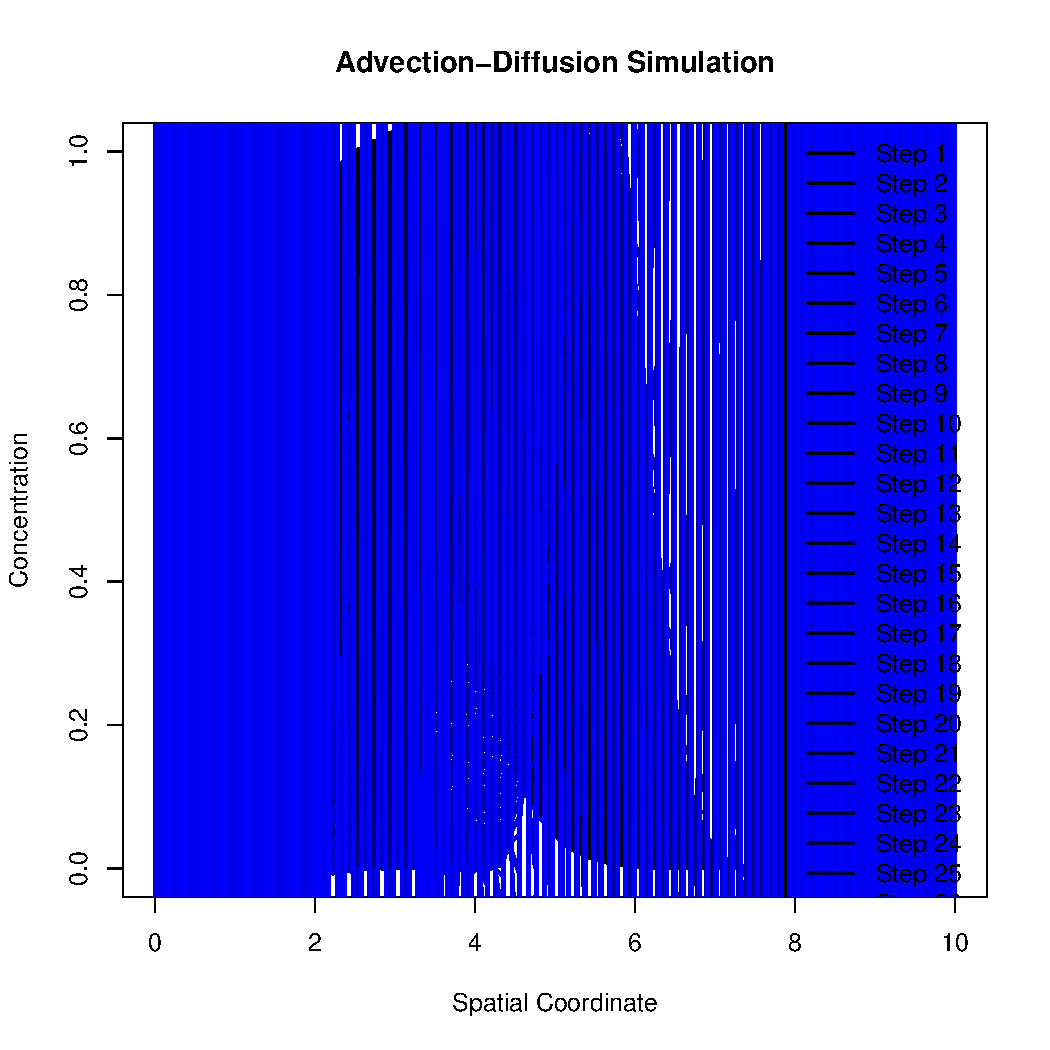
\includegraphics[width=\maxwidth]{figure/unnamed-chunk-3-1} 
\end{knitrout}

This code defines a one-dimensional domain and simulates the advection and diffusion of a concentration field over time using a finite difference method. The initial condition is a Gaussian-shaped concentration profile, and the simulation updates the concentration based on advection and diffusion at each time step. The resulting animation shows the evolution of the concentration profile over time. You can adjust the parameters (e.g., diffusion coefficient, advection coefficient, grid size, time steps) to see how they affect the simulation.


\begin{knitrout}
\definecolor{shadecolor}{rgb}{0.969, 0.969, 0.969}\color{fgcolor}\begin{kframe}
\begin{alltt}
\hlcom{# Model 2 dimensional advection-diffusion using finite difference method}

\hlcom{## set up boundaries}
\hlstd{L} \hlkwb{<-} \hlnum{10}
\hlstd{Nx} \hlkwb{<-} \hlnum{100}
\hlstd{Ny} \hlkwb{<-} \hlnum{100}
\hlstd{dx} \hlkwb{<-} \hlstd{L} \hlopt{/} \hlstd{(Nx} \hlopt{-} \hlnum{1}\hlstd{)}
\hlstd{dy} \hlkwb{<-} \hlstd{L} \hlopt{/} \hlstd{(Ny} \hlopt{-} \hlnum{1}\hlstd{)}
\hlstd{dt} \hlkwb{<-} \hlnum{0.1}
\hlstd{Nt} \hlkwb{<-} \hlnum{100}

\hlcom{## set up initial conditions}
\hlstd{u} \hlkwb{<-} \hlkwd{matrix}\hlstd{(}\hlnum{0}\hlstd{,} \hlkwc{nrow} \hlstd{= Nx,} \hlkwc{ncol} \hlstd{= Ny)}
\hlstd{u[Nx} \hlopt \hlnum{4}\hlopt{:}\hlstd{(}\hlnum{3} \hlopt{*} \hlstd{Nx} \hlopt \hlnum{4}\hlstd{), Ny} \hlopt \hlnum{4}\hlopt{:}\hlstd{(}\hlnum{3} \hlopt{*} \hlstd{Ny} \hlopt \hlnum{4}\hlstd{)]} \hlkwb{<-} \hlnum{1}

\hlcom{## set up coefficients}
\hlstd{alpha} \hlkwb{<-} \hlnum{0.01}
\hlstd{beta} \hlkwb{<-} \hlnum{0.1}

\hlcom{## plot initial conditions}
\hlkwd{image}\hlstd{(}\hlkwd{seq}\hlstd{(}\hlnum{0}\hlstd{, L,} \hlkwc{length.out} \hlstd{= Nx),} \hlkwd{seq}\hlstd{(}\hlnum{0}\hlstd{, L,} \hlkwc{length.out} \hlstd{= Ny), u,} \hlkwc{col} \hlstd{=} \hlkwd{heat.colors}\hlstd{(}\hlnum{100}\hlstd{),} \hlkwc{xlab} \hlstd{=} \hlstr{"x"}\hlstd{,} \hlkwc{ylab} \hlstd{=} \hlstr{"y"}\hlstd{,} \hlkwc{main} \hlstd{=} \hlstr{"Initial Conditions"}\hlstd{)}
\end{alltt}
\end{kframe}
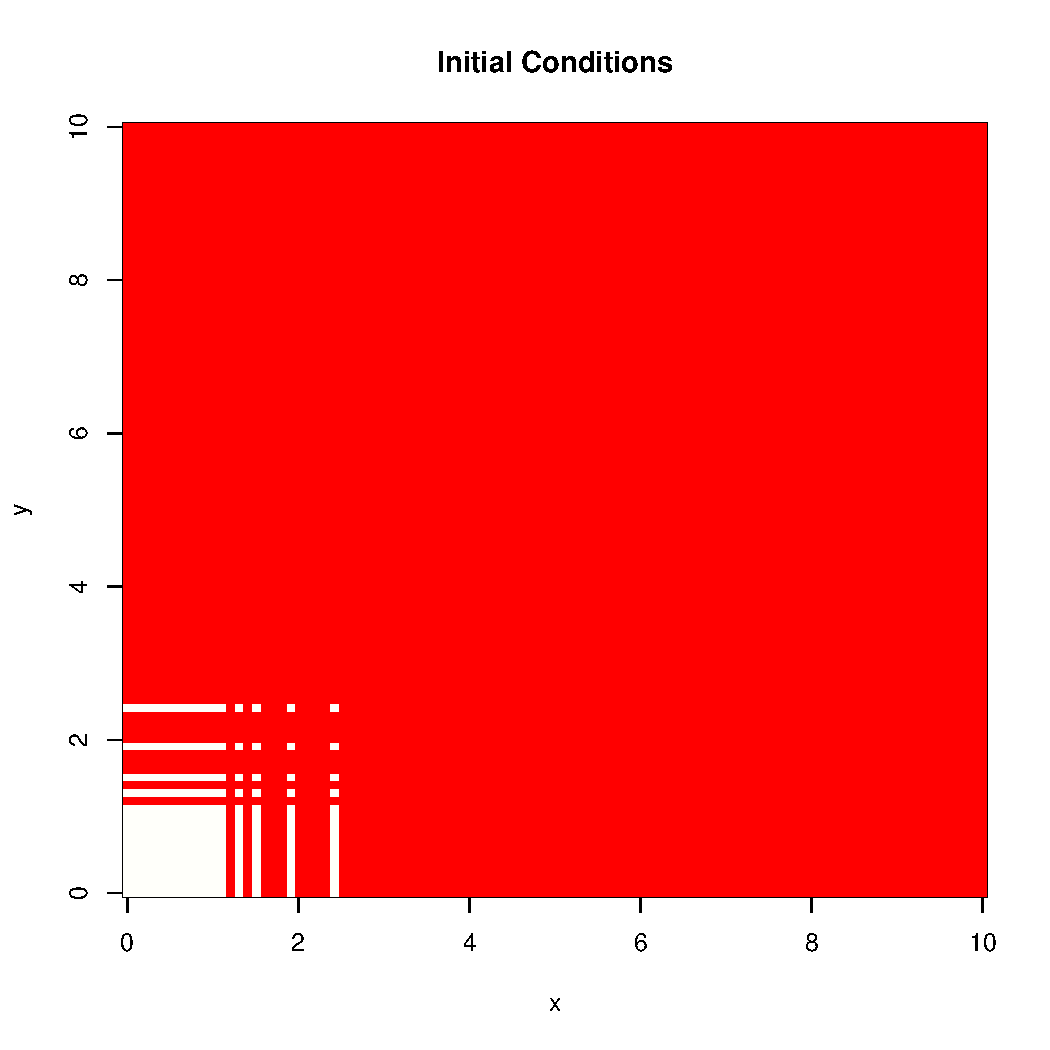
\includegraphics[width=\maxwidth]{figure/unnamed-chunk-4-1} 
\begin{kframe}\begin{alltt}
\hlcom{## simulation loop}
\hlkwa{for} \hlstd{(t} \hlkwa{in} \hlnum{1}\hlopt{:}\hlstd{Nt) \{}
  \hlkwa{for} \hlstd{(x} \hlkwa{in} \hlnum{2}\hlopt{:}\hlstd{(Nx} \hlopt{-} \hlnum{1}\hlstd{)) \{}
    \hlkwa{for} \hlstd{(y} \hlkwa{in} \hlnum{2}\hlopt{:}\hlstd{(Ny} \hlopt{-} \hlnum{1}\hlstd{)) \{}
      \hlstd{u[x, y]} \hlkwb{<-} \hlstd{u[x, y]} \hlopt{+} \hlstd{alpha} \hlopt{*} \hlstd{(u[x} \hlopt{+} \hlnum{1}\hlstd{, y]} \hlopt{-} \hlnum{2} \hlopt{*} \hlstd{u[x, y]} \hlopt{+} \hlstd{u[x} \hlopt{-} \hlnum{1}\hlstd{, y])} \hlopt{*} \hlstd{dt} \hlopt{/} \hlstd{dx}\hlopt{^}\hlnum{2} \hlopt{+} \hlstd{alpha} \hlopt{*} \hlstd{(u[x, y} \hlopt{+} \hlnum{1}\hlstd{]} \hlopt{-} \hlnum{2} \hlopt{*} \hlstd{u[x, y]} \hlopt{+} \hlstd{u[x, y} \hlopt{-} \hlnum{1}\hlstd{])} \hlopt{*} \hlstd{dt} \hlopt{/} \hlstd{dy}\hlopt{^}\hlnum{2} \hlopt{-} \hlstd{beta} \hlopt{*} \hlstd{(u[x} \hlopt{+} \hlnum{1}\hlstd{, y]} \hlopt{-} \hlstd{u[x} \hlopt{-} \hlnum{1}\hlstd{, y])} \hlopt{*} \hlstd{dt} \hlopt{/} \hlstd{(}\hlnum{2} \hlopt{*} \hlstd{dx)} \hlopt{-} \hlstd{beta} \hlopt{*} \hlstd{(u[x, y} \hlopt{+} \hlnum{1}\hlstd{]} \hlopt{-} \hlstd{u[x, y} \hlopt{-} \hlnum{1}\hlstd{])} \hlopt{*} \hlstd{dt} \hlopt{/} \hlstd{(}\hlnum{2} \hlopt{*} \hlstd{dy)}
    \hlstd{\}}
  \hlstd{\}}

  \hlcom{## apply boundary conditions (zero-flux)}
  \hlstd{u[}\hlnum{1}\hlstd{, ]} \hlkwb{<-} \hlstd{u[}\hlnum{2}\hlstd{, ]}
  \hlstd{u[Nx, ]} \hlkwb{<-} \hlstd{u[Nx} \hlopt{-} \hlnum{1}\hlstd{, ]}
  \hlstd{u[,} \hlnum{1}\hlstd{]} \hlkwb{<-} \hlstd{u[,} \hlnum{2}\hlstd{]}
  \hlstd{u[, Ny]} \hlkwb{<-} \hlstd{u[, Ny} \hlopt{-} \hlnum{1}\hlstd{]}

  \hlcom{## plot the current state every 10 time steps}
  \hlkwa{if} \hlstd{(t} \hlopt \hlnum{10} \hlopt{==} \hlnum{0}\hlstd{) \{}
    \hlkwd{image}\hlstd{(}\hlkwd{seq}\hlstd{(}\hlnum{0}\hlstd{, L,} \hlkwc{length.out} \hlstd{= Nx),} \hlkwd{seq}\hlstd{(}\hlnum{0}\hlstd{, L,} \hlkwc{length.out} \hlstd{= Ny), u,} \hlkwc{col} \hlstd{=} \hlkwd{heat.colors}\hlstd{(}\hlnum{100}\hlstd{),} \hlkwc{xlab} \hlstd{=} \hlstr{"x"}\hlstd{,} \hlkwc{ylab} \hlstd{=} \hlstr{"y"}\hlstd{,} \hlkwc{main} \hlstd{=} \hlkwd{paste}\hlstd{(}\hlstr{"Time ="}\hlstd{, t} \hlopt{*} \hlstd{dt))}
    \hlkwd{Sys.sleep}\hlstd{(}\hlnum{0.1}\hlstd{)}  \hlcom{# pause to visualize the animation}
  \hlstd{\}}
\hlstd{\}}
\end{alltt}
\end{kframe}
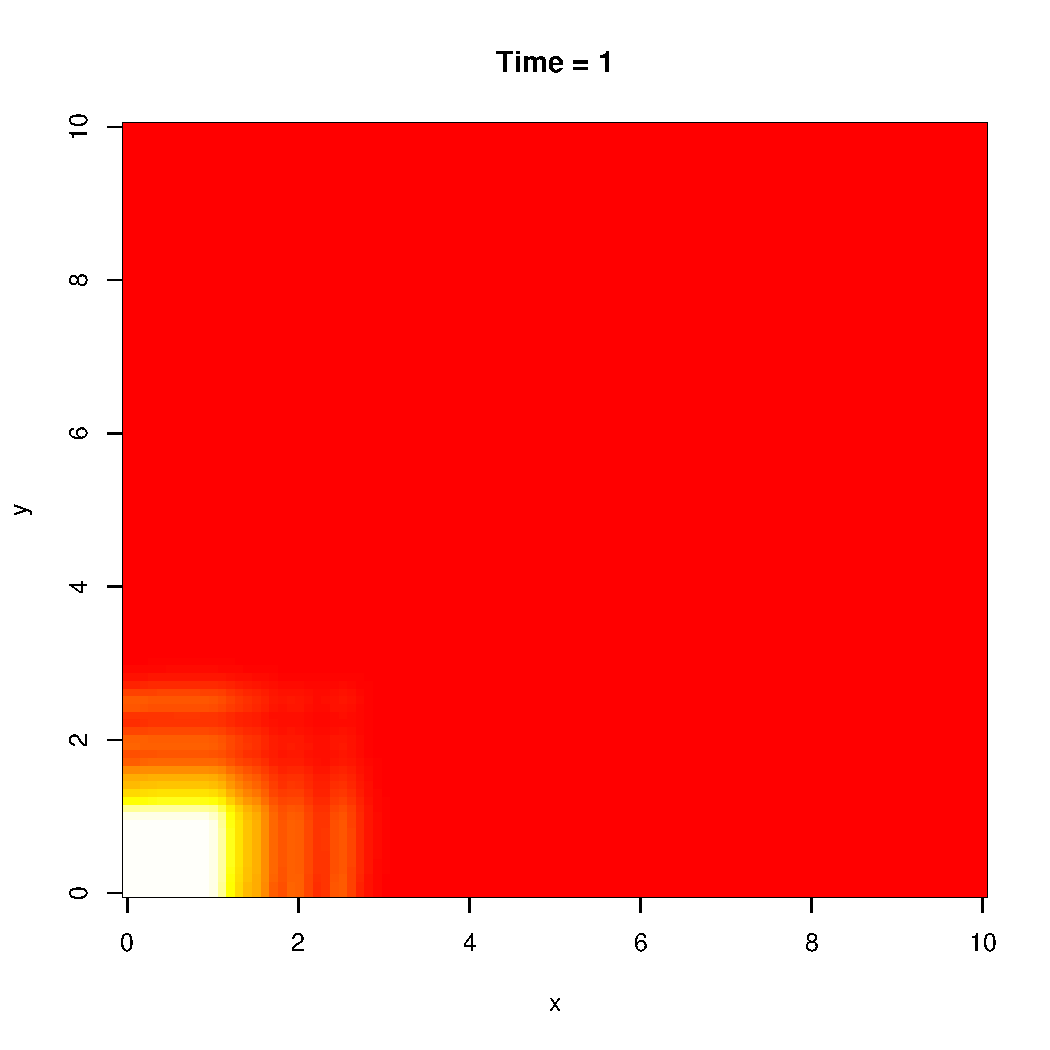
\includegraphics[width=\maxwidth]{figure/unnamed-chunk-4-2} 

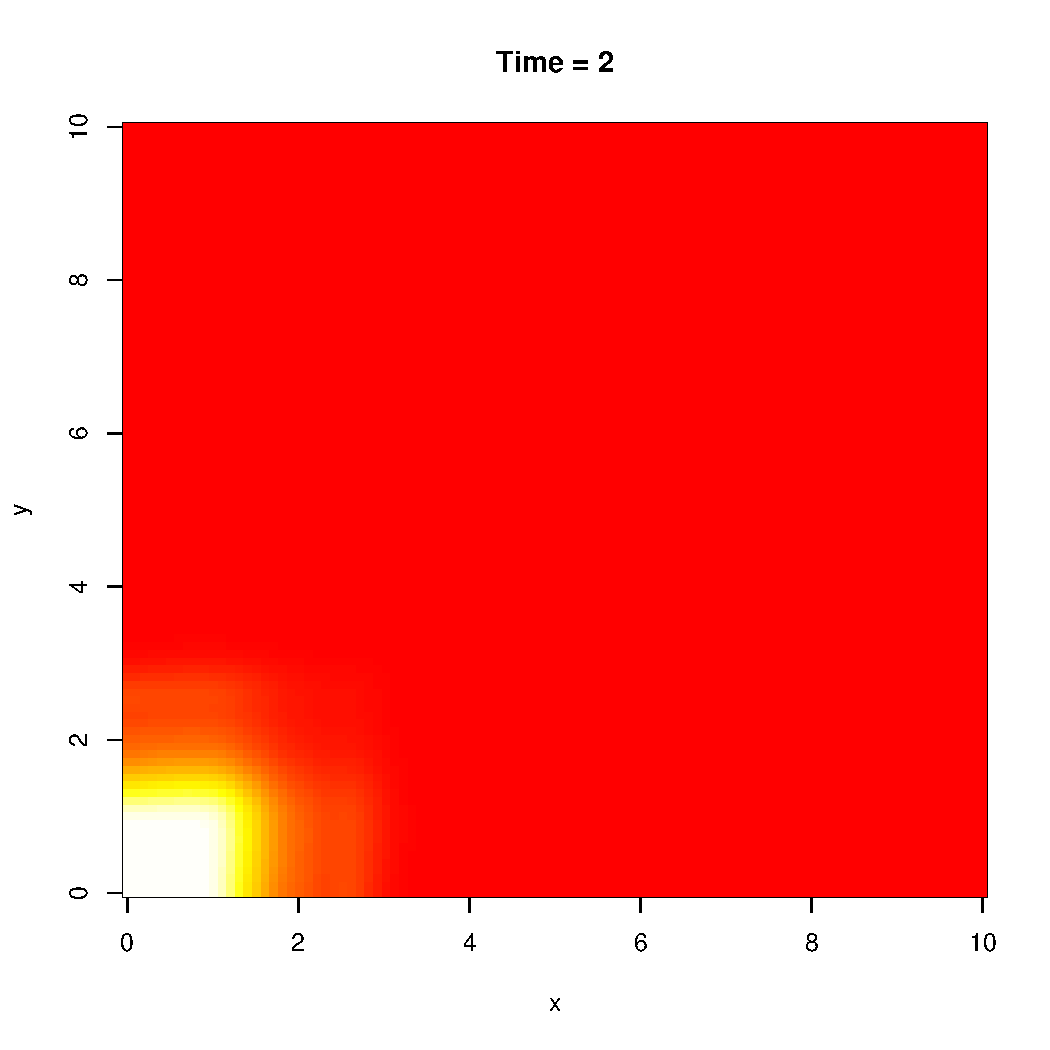
\includegraphics[width=\maxwidth]{figure/unnamed-chunk-4-3} 

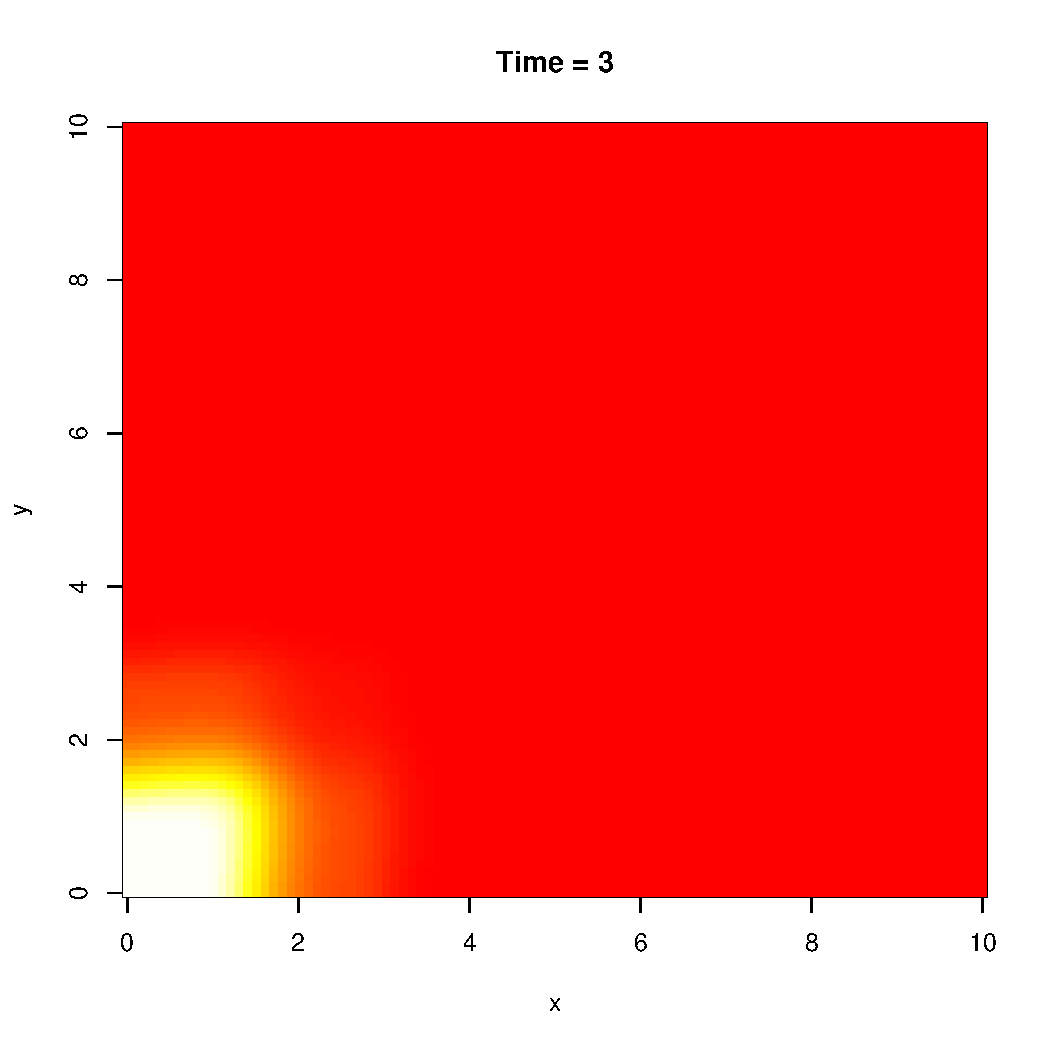
\includegraphics[width=\maxwidth]{figure/unnamed-chunk-4-4} 

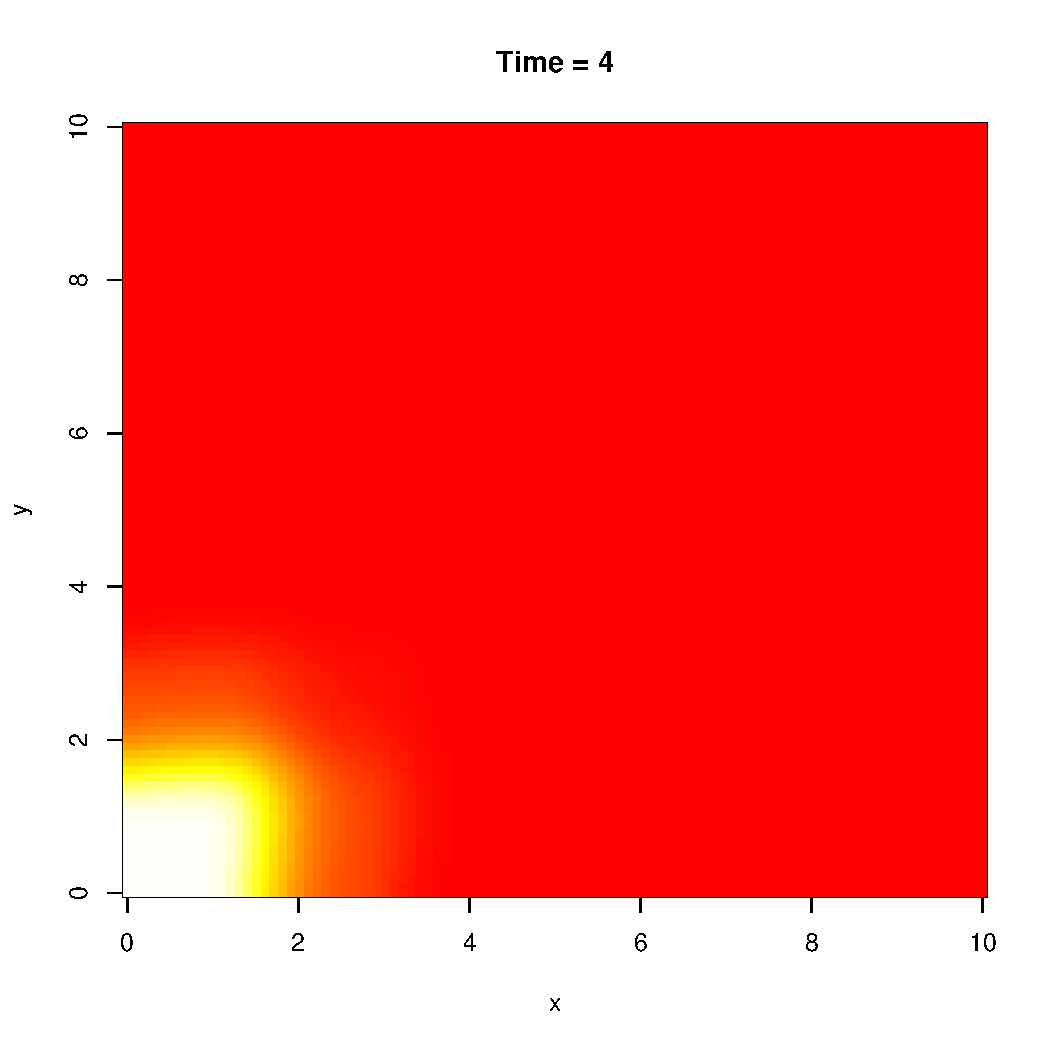
\includegraphics[width=\maxwidth]{figure/unnamed-chunk-4-5} 

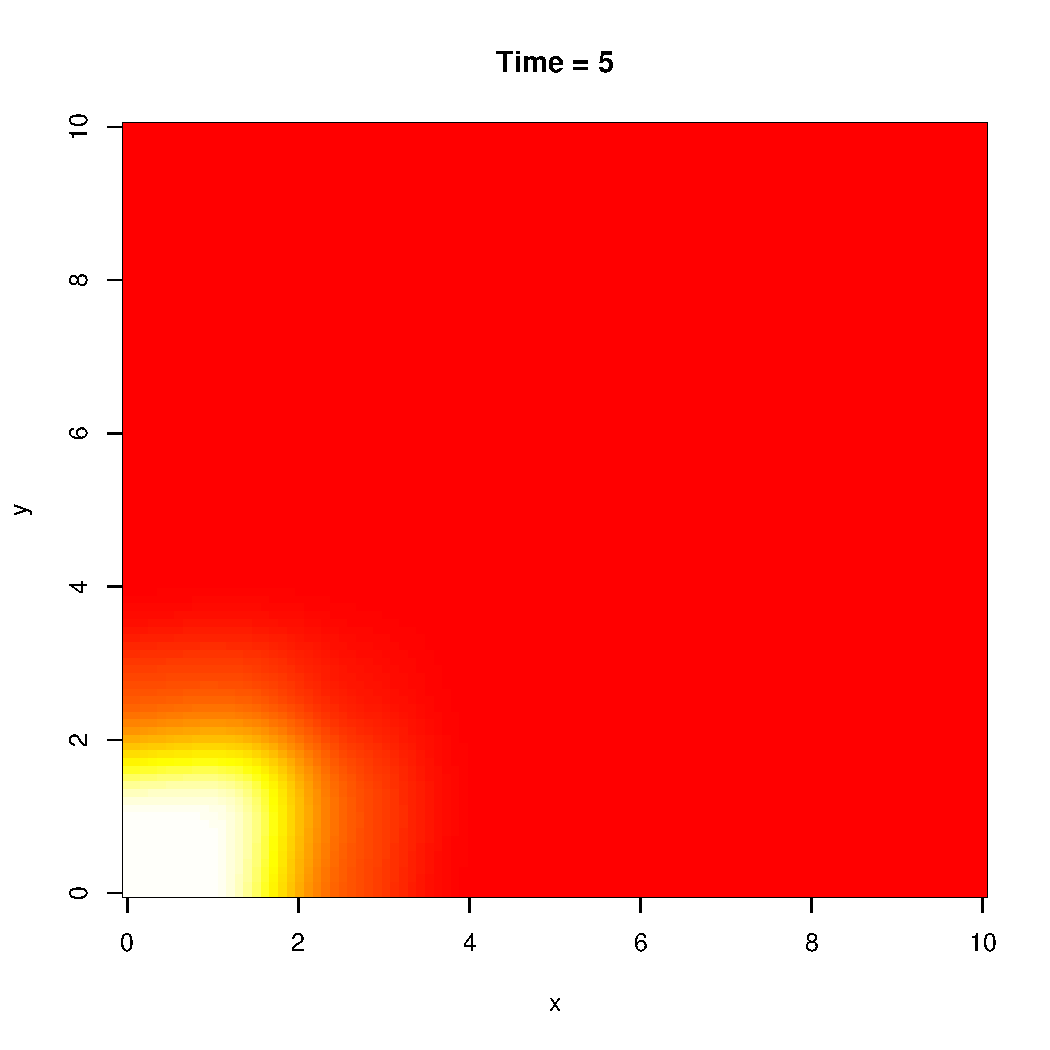
\includegraphics[width=\maxwidth]{figure/unnamed-chunk-4-6} 

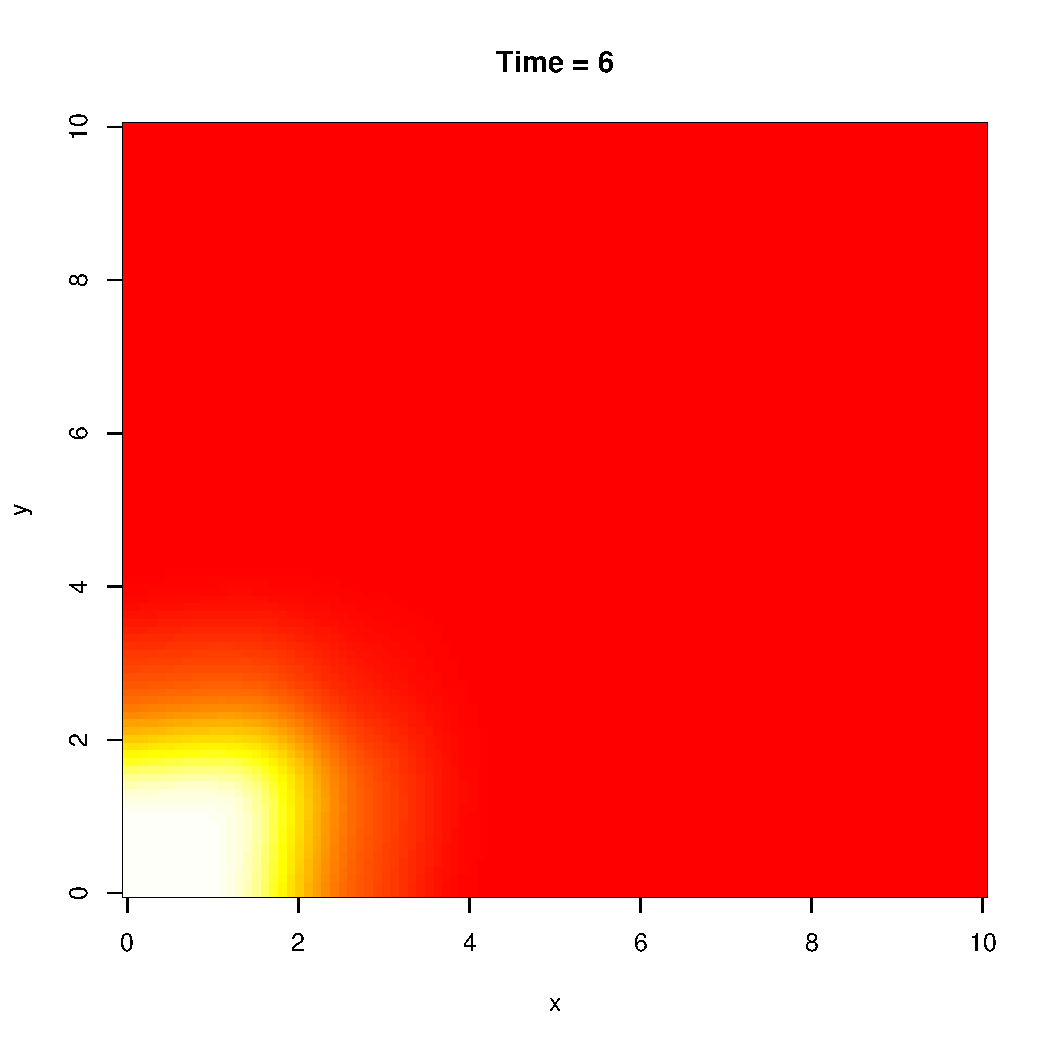
\includegraphics[width=\maxwidth]{figure/unnamed-chunk-4-7} 

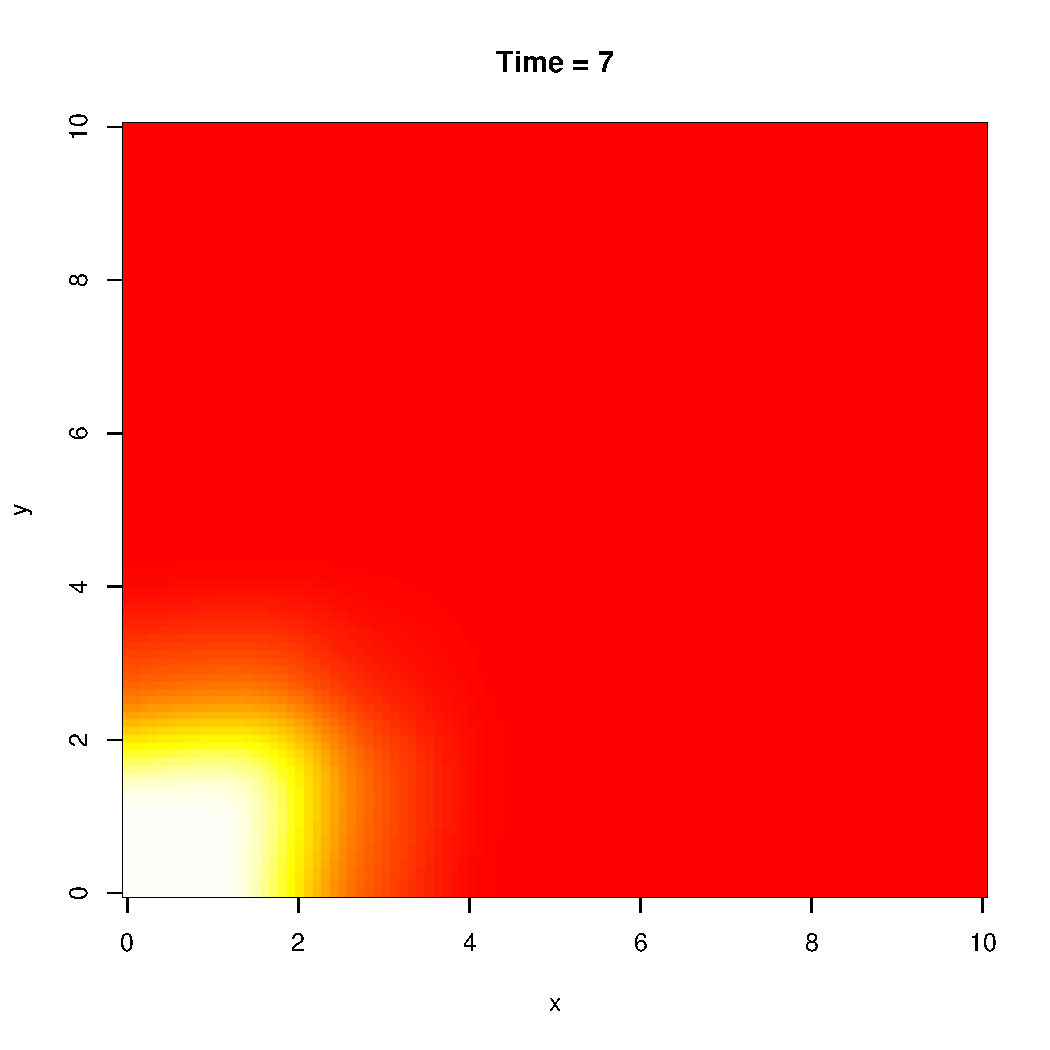
\includegraphics[width=\maxwidth]{figure/unnamed-chunk-4-8} 

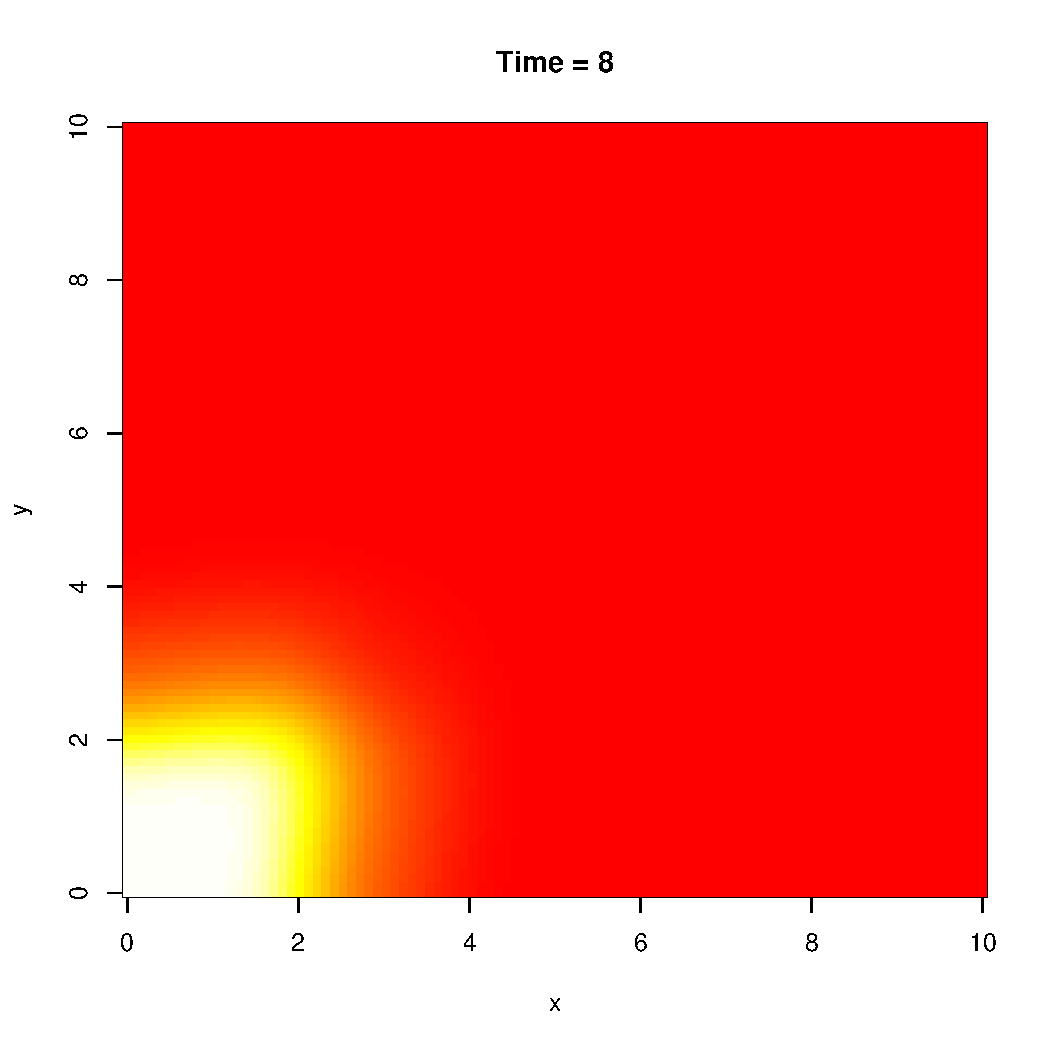
\includegraphics[width=\maxwidth]{figure/unnamed-chunk-4-9} 

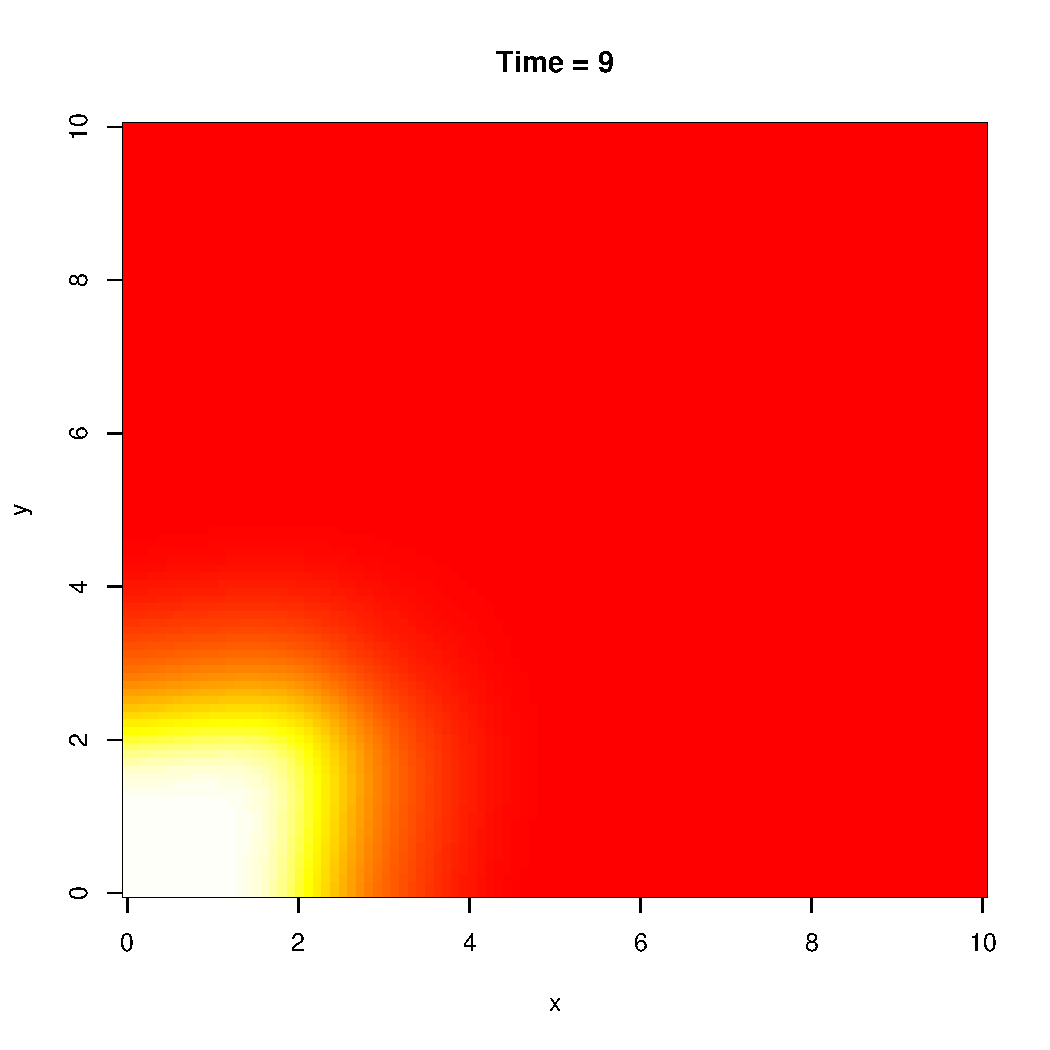
\includegraphics[width=\maxwidth]{figure/unnamed-chunk-4-10} 

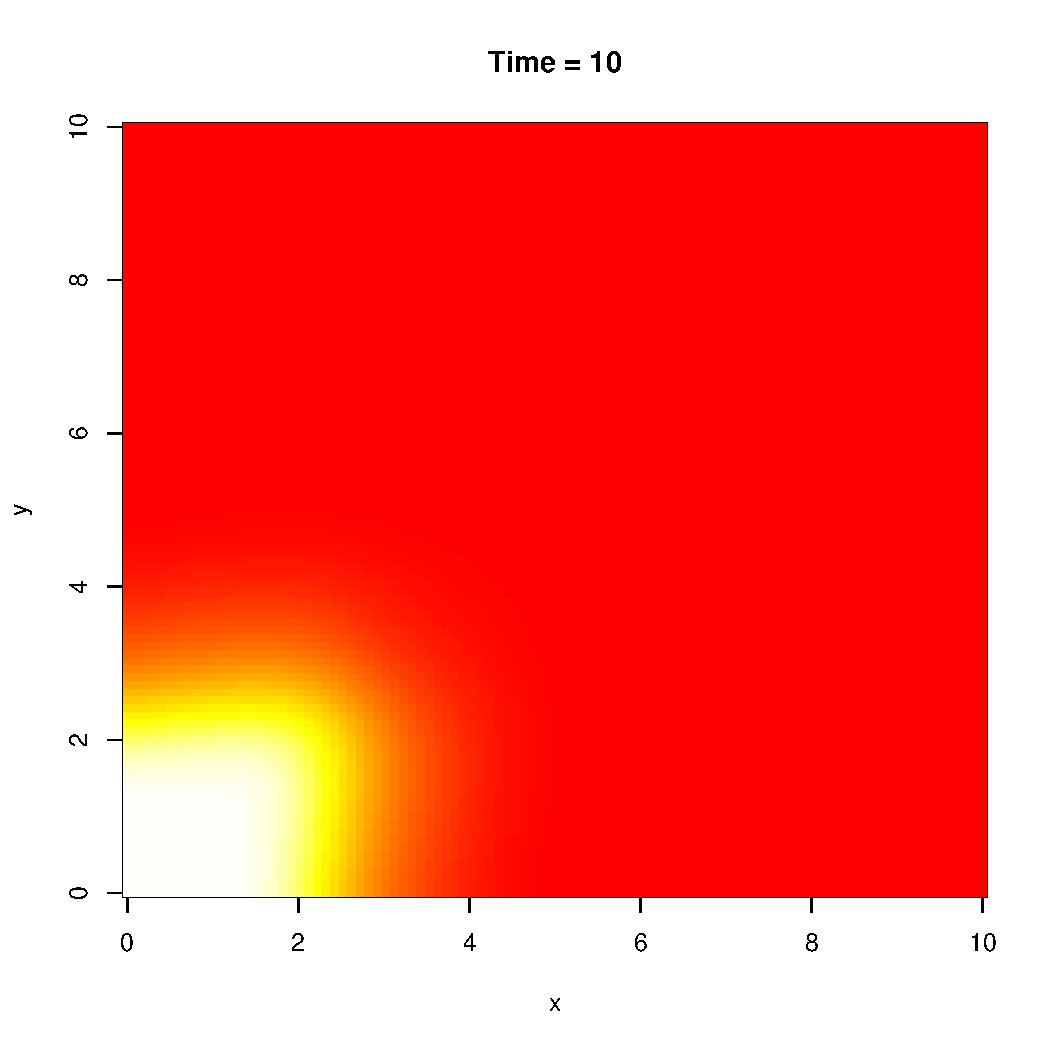
\includegraphics[width=\maxwidth]{figure/unnamed-chunk-4-11} 
\begin{kframe}\begin{alltt}
\hlcom{## plot the final state}
\hlkwd{image}\hlstd{(}\hlkwd{seq}\hlstd{(}\hlnum{0}\hlstd{, L,} \hlkwc{length.out} \hlstd{= Nx),} \hlkwd{seq}\hlstd{(}\hlnum{0}\hlstd{, L,} \hlkwc{length.out} \hlstd{= Ny), u,} \hlkwc{col} \hlstd{=} \hlkwd{heat.colors}\hlstd{(}\hlnum{100}\hlstd{),} \hlkwc{xlab} \hlstd{=} \hlstr{"x"}\hlstd{,} \hlkwc{ylab} \hlstd{=} \hlstr{"y"}\hlstd{,} \hlkwc{main} \hlstd{=} \hlstr{"Final State"}\hlstd{)}
\end{alltt}
\end{kframe}
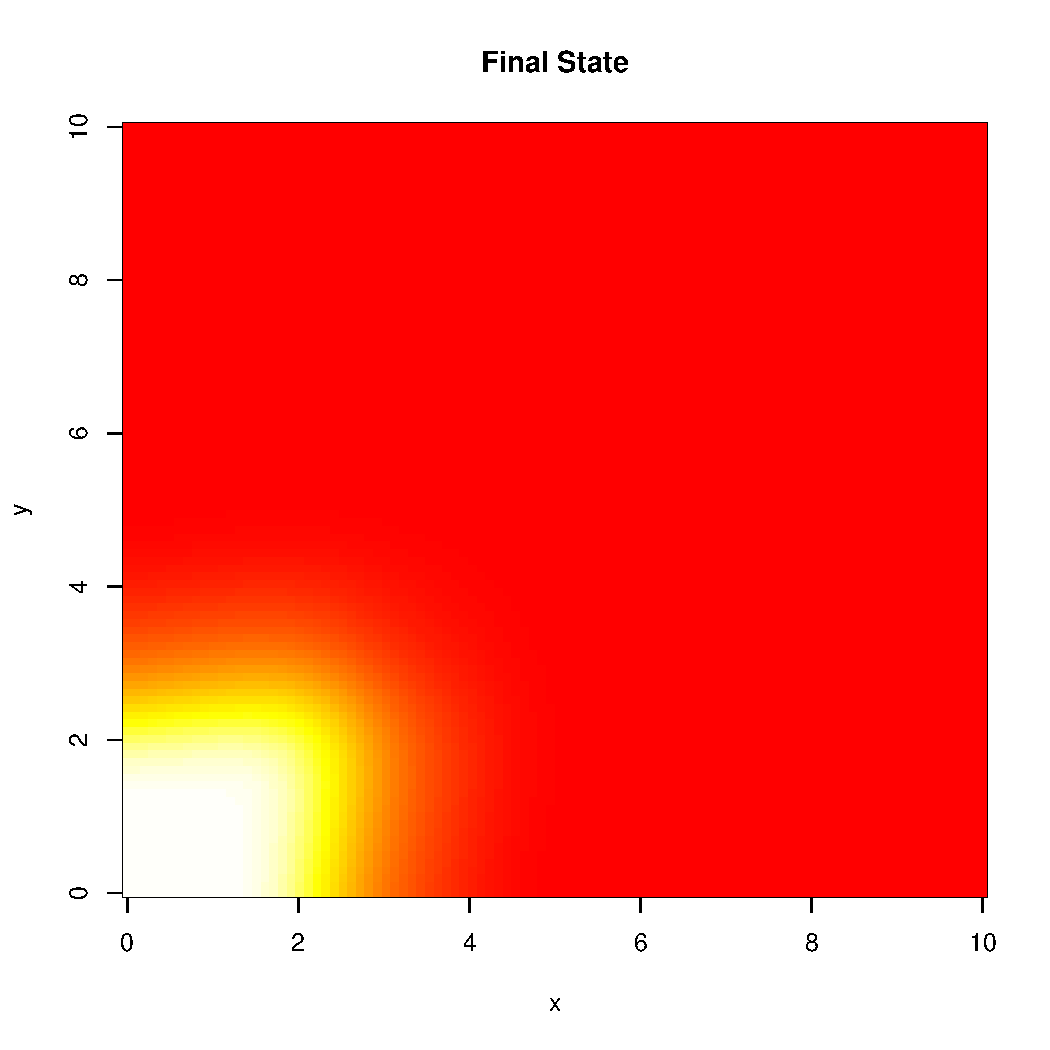
\includegraphics[width=\maxwidth]{figure/unnamed-chunk-4-12} 
\end{knitrout}

\end{document}
